% Options for packages loaded elsewhere
\PassOptionsToPackage{unicode}{hyperref}
\PassOptionsToPackage{hyphens}{url}
\documentclass[
  11pt,
]{article}
\usepackage{xcolor}
\usepackage[margin=22mm]{geometry}
\usepackage{amsmath,amssymb}
\setcounter{secnumdepth}{-\maxdimen} % remove section numbering
\usepackage{iftex}
\ifPDFTeX
  \usepackage[T1]{fontenc}
  \usepackage[utf8]{inputenc}
  \usepackage{textcomp} % provide euro and other symbols
\else % if luatex or xetex
  \usepackage{unicode-math} % this also loads fontspec
  \defaultfontfeatures{Scale=MatchLowercase}
  \defaultfontfeatures[\rmfamily]{Ligatures=TeX,Scale=1}
\fi
\usepackage{lmodern}
\ifPDFTeX\else
  % xetex/luatex font selection
\fi
% Use upquote if available, for straight quotes in verbatim environments
\IfFileExists{upquote.sty}{\usepackage{upquote}}{}
\IfFileExists{microtype.sty}{% use microtype if available
  \usepackage[]{microtype}
  \UseMicrotypeSet[protrusion]{basicmath} % disable protrusion for tt fonts
}{}
\makeatletter
\@ifundefined{KOMAClassName}{% if non-KOMA class
  \IfFileExists{parskip.sty}{%
    \usepackage{parskip}
  }{% else
    \setlength{\parindent}{0pt}
    \setlength{\parskip}{6pt plus 2pt minus 1pt}}
}{% if KOMA class
  \KOMAoptions{parskip=half}}
\makeatother
\usepackage{graphicx}
\makeatletter
\newsavebox\pandoc@box
\newcommand*\pandocbounded[1]{% scales image to fit in text height/width
  \sbox\pandoc@box{#1}%
  \Gscale@div\@tempa{\textheight}{\dimexpr\ht\pandoc@box+\dp\pandoc@box\relax}%
  \Gscale@div\@tempb{\linewidth}{\wd\pandoc@box}%
  \ifdim\@tempb\p@<\@tempa\p@\let\@tempa\@tempb\fi% select the smaller of both
  \ifdim\@tempa\p@<\p@\scalebox{\@tempa}{\usebox\pandoc@box}%
  \else\usebox{\pandoc@box}%
  \fi%
}
% Set default figure placement to htbp
\def\fps@figure{htbp}
\makeatother
\setlength{\emergencystretch}{3em} % prevent overfull lines
\providecommand{\tightlist}{%
  \setlength{\itemsep}{0pt}\setlength{\parskip}{0pt}}
\usepackage{bookmark}
\IfFileExists{xurl.sty}{\usepackage{xurl}}{} % add URL line breaks if available
\urlstyle{same}
\hypersetup{
  hidelinks,
  pdfcreator={LaTeX via pandoc}}

\author{}
\date{}

\begin{document}

\section{The matrix Weyl index in the original phase
coordinates}\label{the-matrix-weyl-index-in-the-original-phase-coordinates}

\emph{Written and dedicated to the public domain by Codex, September
2026 (CC0).}

The preceding lesson constructed the full compact relative projector
from both ordered Weyl errors and compared its classical Chern form with
the cutoff differential form. Here we identify its formal trace using
the exact flat algebra, the original cyclic cocycle and the higher
algebraic index theorem. Two orientation signs arise in different places
and cancel. We then transfer the resulting matrix formula from the
isotropic symbol metric to the original product metric and left
quantization.

Read \href{relative-projectors-chern-cutoff.pdf}{Relative Weyl projectors
and the Chern cutoff form} for (RP1)--(RP16), (CP1)--(CP14) and
(BN1)--(BN5). Read \href{radial-symbol-index-transport.pdf}{Radial
compression and index transport for product-metric symbols} for the full
RC/PT endpoint argument. The \href{scaled-weyl-index-degree.pdf}{Scaled
Weyl parametrices and the surviving differential degree} lesson defines
the separate finite ordered Weyl coefficient; the present source-theorem
route proves its integrated value without deleting any of its terms. The
\href{weyl-trace-criterion.pdf}{Weyl kernels, operator traces, and a
finite trace-class test} lesson fixes the original \((2\pi)^{-n}\)
operator-trace normalization.

The external theorem used below is the higher algebraic index theorem of
M. Pflaum, H. Posthuma and X. Tang. Its degree-zero specialization is
stated at the point of use with the actual compact relative pair and
full curvature. The local top Riemann--Roch input cited in their proof
is due to B. Feigin, G. Felder and B. Shoikhet. Our proof here
establishes the exact product map, cocycle value, characteristic side
and analytic receiving map for the original course symbols.

\subsection{1. The full source product and flat
connection}\label{the-full-source-product-and-flat-connection}

\subsubsection{1.1 The full product and parameter
dictionary}\label{the-full-product-and-parameter-dictionary}

Keep the original phase-space coordinates
\(z=(x_1,\xi_1,\ldots,x_n,\xi_n)\), original orientation
\(\Omega_{\mathrm{AN}}=\bigwedge_{j=1}^n(dx_j\wedge d\xi_j)\), full
matrix product order and formal parameter \(\lambda\). The full
compact-symbol product is: \[
 f\#_\lambda g
 =\sum_{k\ge0}\frac{\lambda^k}{(2i)^k k!}
  \left[
   \sum_{j=1}^n
    \bigl(\partial_{\xi_j}\otimes\partial_{x_j}
          -\partial_{x_j}\otimes\partial_{\xi_j}\bigr)
  \right]^k(f\otimes g)\big|_{\mathrm{matrix\ multiplication}}.
 \tag{FM1}
\] The source writes \(\omega=\sum_jdp_j\wedge dq_j\) and \[
 u\star_\hbar v
 =\sum_{k\ge0}\frac{\hbar^k}{2^k k!}
  \left[
   \sum_{j=1}^n
    \bigl(\partial_{p_j}\otimes\partial_{q_j}
          -\partial_{q_j}\otimes\partial_{p_j}\bigr)
  \right]^k(u\otimes v)\big|_{\mathrm{matrix\ multiplication}}.
 \tag{FM2}
\] For smooth compact symbols, (FM2) means the coefficientwise extension
of the source's polynomial product: at each fixed \(k\) it contains
finitely many derivatives, so it is defined without asserting
convergence of the infinite \(\hbar\)-series.

Define the coordinate swap and coefficientwise parameter substitution \[
 F(x,\xi)=(p=\xi,q=x),\qquad
 \lambda=i\hbar,\qquad
 (\Phi f)(p,q;\hbar)=f(q,p;i\hbar).
 \tag{FM3}
\] This is an isomorphism of Laurent coefficient rings because
\(i\ne0\). The source bidifferential operator in (FM2), acting on
\(\Phi f\otimes\Phi g\), is exactly this course operator in (FM1) after
\(x=q,\xi=p\). Also \((i\hbar)^k/(2i)^k=\hbar^k/2^k\) for every
nonnegative \(k\). The matrix factors remain in their written order.
Thus \textbf{each} finite coefficient agrees, including \(k=0\) and
every noncommutative derivative word: \[
 \Phi(f\#_\lambda g)
   =(\Phi f)\star_\hbar(\Phi g).
 \tag{FM4}
\] The inverse is \((\Phi^{-1}u)(x,\xi;\lambda)=u(\xi,x;\lambda/i)\).
Hence (FM4) is an algebra isomorphism of the actual formal smooth
matrix-symbol algebras, not merely a comparison of their first Poisson
brackets.

The support statement is equally exact. Every term of either product is
a local differential expression, so for coefficientwise compact \(f,g\),
\[
 \operatorname{supp}(\Phi f)=F(\operatorname{supp}f),\qquad
 \operatorname{supp}(f\#_\lambda g)
   \subseteq\operatorname{supp}f\cap\operatorname{supp}g .
 \tag{FM5}
\] The first equality uses the inverse linear diffeomorphism and nonzero
parameter substitution; the second applies coefficient by coefficient.
No completion changes the original support.

\subsubsection{1.2 One exact flat Fedosov realization with the negative
curvature}\label{one-exact-flat-fedosov-realization-with-the-negative-curvature}

The source describes its general Fedosov curvature as the \textbf{full}
closed formal form
\(\Omega_F=-\omega+\hbar\omega_1+\hbar^2\omega_2+\cdots\),
CyclicWeyl.tex lines 365--376. To see concretely that the product (FM2)
has a flat Fedosov realization whose curvature retains the stipulated
negative leading term, take the trivial Weyl bundle over the same
\((p,q)\)-space. Write \(P_j,Q_j\) for fiber coordinates, with the
\textbf{same} fiber product (FM2), so
\([P_j,Q_k]_\star=\hbar\delta_{jk}\). Use the flat base connection
\(d_{p,q}\), zero curvature \(\widetilde R=0\), and the explicit
one-form \[
 A_0=\sum_j(Q_j\,dp_j-P_j\,dq_j),\qquad
 B=-2\sum_jp_j\,dq_j,\qquad A=A_0+B .
 \tag{FM6}
\] Here \(B\) is central in the fiber Weyl algebra; it changes the
chosen curvature representative but contributes nothing to the
commutator derivation. For every fiber section \(U\), \[
 D U=d_{p,q}U+\hbar^{-1}[A,U]_\star
 =\sum_j\left[
   dp_j(\partial_{p_j}-\partial_{P_j})U
  +dq_j(\partial_{q_j}-\partial_{Q_j})U
 \right].
 \tag{FM7}
\] Indeed \([Q_j,U]_\star=-\hbar\partial_{P_j}U\) and
\([P_j,U]_\star=\hbar\partial_{Q_j}U\) exactly: a linear fiber
coordinate has no second or higher derivatives. Thus (FM7) has no hidden
higher-order term. Its unique horizontal lift with value
\(u(p,q;\hbar)\) at \(P=Q=0\) is the coefficientwise Taylor section
\(\widehat u(p,q;P,Q;\hbar)=u(p+P,q+Q;\hbar)\); direct substitution into
(FM7) gives \(D\widehat u=0\).

The source curvature formula for the flat base connection is
\(\Omega_F=dA+(2\hbar)^{-1}[A,A]_\star\), with the \textbf{graded}
bracket of one-forms. Since \(P,Q\) are fiber variables independent of
the base, \(dA_0=0\). The central \(B\) satisfies \(dB=-2\omega\) and
has no graded commutator contribution. The remaining product is \[
 \hbar^{-1}A_0\wedge_\star A_0
 =\hbar^{-1}\sum_j
   \bigl((-Q_j)\star P_j+P_j\star Q_j\bigr)\,dp_j\wedge dq_j
 =\hbar^{-1}\sum_j[P_j,Q_j]_\star\,dp_j\wedge dq_j
 =\omega .
 \tag{FM8}
\] In the first displayed coefficient, \((-Q_j)\star P_j+P_j\star Q_j\)
is exactly \([P_j,Q_j]_\star\); all cross-index contributions cancel by
the separate coordinate commutators. Consequently \[
 \Omega_F=-2\omega+\omega=-\omega,\qquad
 D^2=\hbar^{-1}[\Omega_F,-]_\star=0 .
 \tag{FM9}
\] This explicit representative has all higher \(\omega_j=0\). The full
general source curvature remains in (FC4)--(FC7); the central shift
stays in the cocycle computation below.

The central term is a choice of lift of the derivation-valued
connection, not a degree-zero perturbation of its noncentral Fedosov
correction. The source's exact derivation sequence in CyclicWeyl.tex
lines 37--43 has the constants as kernel. In the present flat model the
actual derivation is \(d-\delta\) in (FM7), with zero higher noncentral
correction. Both \(A_0\) and \(A_0+B\) give this same derivation and
hence the same horizontal algebra at every coefficient. The antecedent
FFSrevised.tex lines 2189--2194 expressly permits a central one-form
change of this lift before choosing its Chern--Weil representative. We
keep the complete \(A_0+B\), including \(dB=-2\omega\), rather than
identify the two curvature forms pointwise.

For the particular degree-zero pairing used here, the equality of the
trace densities under this central change is also direct. In the full
determinant contraction (WR9), every one of the \(2n\) connection slots
is differentiated once in a fiber coordinate. Any term with \(B\) in one
such slot vanishes because \(B\) is fiber constant. Thus the complete
cochain on \(A_0+B\) equals that on \(A_0\); no matrix word or
noncentral term is removed. On the characteristic side the two closed
curvature representatives are \(\Omega_0=+\omega\) and
\(\Omega_1=-\omega=\Omega_0+dB\). For the full compact closed relative
Chern form \(\gamma\) of (FC3), put \(\Omega_s=\Omega_0+s\,dB\). The
exact transgression, retaining the full exponential and its inverse
parameter, is

\[
 \frac{d}{ds}\bigl[\gamma\wedge
     e^{-\Omega_s/(2\pi i\hbar)}\bigr]_{2n}
 =d\left[-\frac{1}{2\pi i\hbar}\,\gamma\wedge B\wedge
     e^{-\Omega_s/(2\pi i\hbar)}\right]_{2n-1}.
 \tag{FC8}
\]

Indeed \(d\gamma=0=d\Omega_s\), every degree of \(\gamma\) is even, and
\(dB\) commutes with the other two-forms; differentiating the finite
top-degree exponential gives exactly the displayed factor. The
rank-difference term of \(\gamma\) is identically zero, and every
remaining coefficient has the original compact support \(K\). The
primitive in (FC8) is therefore compactly supported despite the
noncompact \(B\). Stokes followed by integration over \(s\in[0,1]\)
proves equality of the two characteristic integrals, coefficient by
coefficient. Consequently the source pairing on the actual flat
connection and the source negative-curvature representative used in
(MB3) agree by an explicit cochain calculation and an exact compact
transgression. No assumption that the central term belongs to the
source's degree-at-least-three noncentral correction is needed.

For horizontal lifts, fiber differentiation of \(\widehat u\) is base
differentiation of \(u\). Therefore \[
 \widehat u\star_{\mathrm{fiber}}\widehat v
 =\widehat{u\star_\hbar v},\qquad
 (\widehat u\star_{\mathrm{fiber}}\widehat v)|_{P=Q=0}
 =u\star_\hbar v .
 \tag{FM10}
\] This establishes the source-form Fedosov product for the explicit
connection at \textbf{every} formal order and shows why (FM4), not an
assumed gauge equivalence, is the exact algebra map used below.

\subsubsection{1.3 Transport of the actual compact relative
projector}\label{transport-of-the-actual-compact-relative-projector}

Let \(e_\infty,e_0\in M_{2\nu}\) be the specific formal idempotents of
RP11, built from the original ordered \(a,b=\psi a^{-1}\) and both error
sides. RP11 proves \[
 e_\infty\#_\lambda e_\infty=e_\infty,\qquad
 e_0\#_\lambda e_0=e_0,\qquad
 \operatorname{supp}(e_\infty-e_0)_k
  \subseteq K:=\operatorname{supp}(1-\psi)
 \quad\text{for every coefficient }k .
 \tag{FM11}
\] Apply (FM4) to the \textbf{whole} matrix idempotents, not merely to
their zeroth terms. With \(E_\infty=\Phi e_\infty\) and
\(E_0=\Phi e_0\), one obtains \[
 E_\infty\star_\hbar E_\infty=E_\infty,\qquad
 E_0\star_\hbar E_0=E_0,\qquad
 \operatorname{supp}(E_\infty-E_0)_k\subseteq F(K).
 \tag{FM12}
\] The reference rank, all original matrix off-diagonal terms, powers of
\(i\), and both original error orders survive. The horizontal-lift map
of (FM7)--(FM10) realizes \(E_\infty,E_0\) as flat Fedosov idempotents
for this explicit connection. Their difference is coefficientwise
compact in the same fixed set \(F(K)\), so every local source density
evaluated \textbf{on the difference} has a legitimate compact support.
This supplies the actual compact relative pair to the source theorem.

The orientation remains separate from the algebra map: \[
 F^*(\omega^n/n!)=(-1)^n\Omega_{\mathrm{AN}},\qquad
 \deg_{\mathrm{or}}F=(-1)^n .
 \tag{FM13}
\]

\subsection{2. Degree-zero pairing and the exact cyclic
sign}\label{degree-zero-pairing-and-the-exact-cyclic-sign}

Let \(\Psi=\Psi_{2n}^{2n}\) be the source trace density of
CyclicWeyl.tex definition dfn:psi. For a compactly supported flat formal
symbol \(f\), use the source's own integral functional, as written in
HAnaInThm.tex lines 541--548: \[
 T_\Psi(f):=\int_M\Psi(f).
 \tag{NS1}
\] The source's definition dfn:chi, at \(i=r=0\) and \(\alpha_0=1\),
gives directly \[
 \chi_{0,M}^{0}(1)(f)
   =\int_M1\wedge\Psi_{2n}^{2n}(f)
   =T_\Psi(f).
 \tag{NS2}
\] Its subsequent construction, CyclicWeyl.tex equation consmor2,
includes the explicit factor \((2\pi\sqrt{-1})^{-n}\). At degree zero
there is one summand, so no cyclic-periodicity convention or higher
cochain can change the following exact identity: \[
 \mathsf Q_M^0(1)(f)
   =\frac{1}{(2\pi i)^n}\chi_{0,M}^{0}(1)(f)
   =\frac{1}{(2\pi i)^n}T_\Psi(f).
 \tag{NS3}
\] This statement uses only the source definitions and is valid for the
compact-support algebra on the actual flat \(M=\mathbb R^{2n}\). The
source extends the Weyl cocycles to finite matrices by the ordered
ordinary trace, IndThms.tex lines 163--171. Thus (NS3) holds with \(f\)
replaced by a compactly supported matrix symbol and \(T_\Psi\) replaced
by its matrix-trace extension.

For the relative pair \((e_\infty,e_0)\) of the preceding lesson, the
difference is coefficientwise supported in the fixed compact
\(K=\operatorname{supp}(1-\psi)\). Locality of \(\Psi\) keeps its
evaluation on the difference supported there. At cyclic degree zero, the
source Chern chain is exactly \(c_0(e)=e\), IndThms.tex lines 21--44;
the higher \(c_j\) do not enter. By linearity and the source pairing
definition at lines 123--134, \[
 \big\langle\mathsf Q^0(1),e_\infty-e_0\big\rangle
  =\frac{1}{(2\pi i)^n}
      \int_{\mathbb R^{2n}}
        \Psi^{(2\nu)}(e_\infty-e_0).
 \tag{NS4}
\] No finite-parametrix error, matrix order, rank reference or support
term has been discarded. Equation (NS4) is the exact source cyclic
pairing-to-source trace-density morphism needed before a comparison with
RP16.

\subsubsection{2.1 The operator that the source's proof
specifies}\label{the-operator-that-the-sources-proof-specifies}

Write \(z_{2s-1}=P_s,z_{2s}=Q_s\) for \(1\leq s\leq n\). On \(2k\)
ordered tensor slots \(r=0,\ldots,2k-1\), let
\(D_{ra}=\partial_{z_a}^{(r)}\). All the \(D_{ra}\) commute, even when
different partial derivatives act on the same slot. The source's Poisson
operator is \[
 \alpha_{rs}=\sum_{\ell=1}^n
 (D_{r,2\ell-1}D_{s,2\ell}
  -D_{r,2\ell}D_{s,2\ell-1}),\qquad
 \alpha_{sr}=-\alpha_{rs}.
 \tag{WR1}
\] The plus sign before the displayed minus is ordinary addition; no
\(1/2\) is included in \(\alpha\). For a \(k\)-element subset
\(I\subset\{1,\ldots,n\}\), let \(D_I\) be the \(2k\)-by-\(2k\) matrix
with rows the tensor slots and columns \(P_\ell,Q_\ell\) for
\(\ell\in I\), in increasing plane order. Define the full alternating
operator \[
 \Pi_{2k}^{[n]}=\sum_{\substack{I\subset\{1,\ldots,n\}\\|I|=k}}
       \det D_I,\qquad
 \Pi_0^{[n]}=1,\qquad
 \Pi_{2k}^{[n]}=0\quad(k>n).
 \tag{WR2}
\] For \(k=n\), this is precisely the full determinant with its slots
relabelled \(0,\ldots,2n-1\), including every one of the \((2n)!\)
signed permutations and no factorial multiplier. The superscript \([n]\)
records the \emph{ambient} number of symplectic planes; it is not a
matrix rank.

Here is an exact operator identity for \(0\leq k<n\). Let
\((\Pi_{2k}^{[n]})^i\) act on the \(2k\) ordered slots of a
\(2k+2\)-slot tensor other than slots \(0\) and \(i\). Then \[
 \boxed{\quad
 \Pi_{2k+2}^{[n]}
 =\sum_{i=1}^{2k+1}(-1)^i
       \alpha_{i0}(\Pi_{2k}^{[n]})^i .
 \quad}
 \tag{WR3}
\] To prove it without a normalization convention, introduce exterior
basis symbols \(e_0,\ldots,e_{2k+1}\) over the commutative ring
generated by the \(D_{ra}\). Put \(v_a=\sum_r D_{ra}e_r\). Direct
expansion of (WR1) gives \[
 \beta:=\sum_{r<s}\alpha_{rs}e_r\wedge e_s
      =\sum_{\ell=1}^{n}v_{2\ell-1}\wedge v_{2\ell}.
 \tag{WR4}
\] In \(\beta^{k+1}/(k+1)!\), the square of each decomposable plane term
vanishes. A set \(I\) of \(k+1\) \emph{distinct} planes occurs
\((k+1)!\) times before division. The coefficient of
\(e_0\wedge\cdots\wedge e_{2k+1}\) is therefore
\(\sum_{|I|=k+1}\det D_I=\Pi_{2k+2}^{[n]}\). Equivalently, this
coefficient is the Pfaffian of the skew matrix \((\alpha_{rs})\), with
its fully written normalization \[
 \operatorname{Pf}_{2k+2}(\alpha)
 =\frac{1}{2^{k+1}(k+1)!}
   \sum_{\sigma\in S_{2k+2}}\operatorname{sgn}(\sigma)
   \prod_{j=1}^{k+1}
      \alpha_{\sigma(2j-2),\sigma(2j-1)} .
 \tag{WR5}
\] This follows directly by expanding \(\beta^{k+1}\): each pairing
appears in \(2^{k+1}(k+1)!\) ordered and internally oriented forms.
Sorting the pair containing slot \(0\) gives the Pfaffian Laplace
expansion \[
 \operatorname{Pf}_{2k+2}(\alpha)
 =\sum_{i=1}^{2k+1}(-1)^{i+1}
       \alpha_{0i}\operatorname{Pf}_{2k}(\alpha_{\widehat0\widehat i}).
 \tag{WR6}
\] The removed-slot Pfaffian equals \((\Pi_{2k}^{[n]})^i\) by the same
(WR4) calculation on those ordered remaining slots. Since
\(\alpha_{0i}=-\alpha_{i0}\), (WR6) is exactly (WR3). This proof also
shows why repeated choices of one symplectic plane cancel rather than
add a hidden \(k!\): their exterior square is zero.

Pflaum--Posthuma--Tang explicitly take
\((\hbar\alpha)^{\wedge1}=\hbar\alpha\) in their one-plane display,
CyclicWeyl.tex lines 124--134. In the proof of
\(b\tau_{2k}=\tau_{2k+1}\), their lines 232--257 assert, on the actual
ordered slots, that \[
 \sum_{i=1}^{2k+1}(-1)^i\hbar\alpha_{i0}
       \big((\hbar\alpha)^{\wedge k}\big)^i
   =(\hbar\alpha)^{\wedge(k+1)} .
 \tag{WR7}
\] They first write the larger \(\sum_s\) expression, then explicitly
identify its \(s=0\) part with the right side; (WR7) is that
identification, not an inferred equality from the theorem alone.
Starting from their displayed degree-one operator, (WR7) uniquely
determines every subsequent power by induction. Equation (WR3),
including the \(k=0\) base \(\alpha_{01}=\Pi_2^{[n]}\), proves the
source-specified power is \[
 \boxed{\quad
  (\hbar\alpha)_{\mathrm{PPT}}^{\wedge k}
       =\hbar^k\Pi_{2k}^{[n]}
       \quad\text{on every ordered set of \(2k\) slots},
       \qquad 0\leq k\leq n .
  \quad}
 \tag{WR8}
\] The source's separate remark at lines 113--115 that its top cocycle
is Feigin--Felder--Shoikhet's up to \((-1)^n\) agrees with (WR8). A
convention using the \emph{undivided} exterior power would instead give
\(k!\Pi_{2k}^{[n]}\), fail (WR7) already at \(k=2\), and disagree with
that top-cocycle remark. The factor of two from an undivided exterior
square at \(k=2\) is thus resolved by the source's own recursion.

\subsubsection{2.2 Exact value of the source cochain for the written
connection}\label{exact-value-of-the-source-cochain-for-the-written-connection}

The source definition at CyclicWeyl.tex lines 95--112 and (WR8), with
the full ordered exponential product \(\mathcal E\), give an equality of
cochains in every dimension: \[
 \tau_{2n}^{\mathrm{PPT}}
   =(-1)^n\hbar^n\mu_{2n}
       \int_{\Delta^{2n}}\mathcal E(u)\Pi_{2n}^{[n]}\,du_1\cdots du_{2n}
   =\tau_{2n}^{\det}.
 \tag{WR9}
\] No \(n!\) is omitted: (WR5) and (WR8) specify it. For the full FM6
connection \[
 A=\sum_{j=1}^n(Q_j\,dp_j-P_j\,dq_j)-2\sum_{j=1}^np_j\,dq_j,
 \quad D=d-\sum_j(dp_j\partial_{P_j}+dq_j\partial_{Q_j}),
 \quad \Omega_F=-\omega,
 \tag{WR10}
\] and each compact formal matrix symbol \(u\), its horizontal section
is \(\widehat u(p,q;P,Q)=u(p+P,q+Q)\). The central shift in \(A\)
supplies the written curvature and has zero fiber derivative; it is
retained, not removed from the connection.

At degree \(2n\), the source shuffle in CyclicWeyl.tex lines 393--411
has a length-zero first chain and only the identity \((0,2n)\)-shuffle.
Its definition of \(\Psi\) at lines 550--570 therefore gives \[
 \Psi_{2n}^{2n}(\widehat u)
  =\hbar^{-2n}\tau_{2n}^{\mathrm{PPT}}
       (\widehat u,A,\ldots,A).
 \tag{WR11}
\] All \(2n\) inverse powers, the ordinary ordered matrix trace and the
full \(A\) are present. By (WR9), this is the source cochain on the
written connection. The determinant contraction can be calculated
without a normalization shortcut:

Write \[
 \beta_{2j-1}:=\partial_{P_j}A=-dq_j,\qquad
 \beta_{2j}:=\partial_{Q_j}A=dp_j .
 \tag{FD5}
\] Each factor \(A\) is differentiated exactly once in every summand of
(the full determinant). Exterior multiplication of the resulting
differential-form slots gives \[
 \begin{aligned}
 \bigwedge \Pi_{2n}
   (\widehat u\otimes A^{\otimes2n})
 &=\widehat u\sum_{\sigma\in S_{2n}}
     \operatorname{sgn}(\sigma)\,
       \beta_{\sigma(1)}\wedge\cdots\wedge\beta_{\sigma(2n)}\\
 &=(2n)!\,\widehat u\,
     \beta_1\wedge\cdots\wedge\beta_{2n}\\
 &=(2n)!\,\widehat u\,
     \bigwedge_{j=1}^n(dp_j\wedge dq_j)
 =(2n)!\,\widehat u\,\frac{\omega^n}{n!}.
 \end{aligned}
 \tag{FD6}
\] The second equality uses the sign of the permutation once from the
determinant and once from exterior permutation, so every one of the
\((2n)!\) summands has the same sign. The third equality retains each
original ordered coordinate pair:
\((-dq_j)\wedge dp_j=dp_j\wedge dq_j\).

After (the full determinant) acts, every \(A\)-slot has fiber-constant
coefficients \(\beta_j\). Every positive-degree term in any exponential
of (the ordered exponential) differentiates one such constant slot and
vanishes, including the terms involving slot zero. Thus \(\mathcal E\)
acts as the identity \textbf{on this exact tensor}. The simplex volume
is \(1/(2n)!\), and \(\mu_{2n}\) evaluates \(\widehat u\) at \(P=Q=0\),
yielding \(u\).

These equations retain all \((2n)!\) permutations, the ordered simplex
volume \(1/(2n)!\), and the vanishing of every positive exponential term
after the \(A\)-slots become fiber-constant. Hence, coefficientwise for
every finite matrix rank \(m\), \[
 \boxed{\quad
 \Psi_{2n}^{2n,(m)}(\widehat u)
 =(-1)^n\hbar^{-n}\operatorname{tr}_m(u)\frac{\omega^n}{n!}.
 \quad}
 \tag{WR12}
\] There is no assumption that \(u\) is scalar, idempotent or only a
zeroth-order symbol. At each formal order the source expression is local
in finitely many derivatives, so a fixed coefficientwise compact support
remains compact.

Retain the source normalization \((2\pi i)^{-n}\), the exact algebra map
\(p=\xi,q=x,\lambda=i\hbar\) of FM3--FM4, and both separate orientation
signs of FM13. Their product is \(+1\) in the phase-space integral. Thus
for every compact formal finite-matrix symbol \(f\) in the original
ordered Moyal algebra, \[
 \boxed{\quad
 \mathsf Q^0(1)(\widehat{\Phi f})
  =(2\pi i)^{-n}\int_{\mathbb R^{2n}_{p,q}}
       \Psi_{2n}^{2n,(m)}(\widehat{\Phi f})
  =(-1)^n(2\pi\lambda)^{-n}
       \int_{\mathbb R^{2n}_{x,\xi}}
           \operatorname{tr}_m(f)\,\Omega_{\mathrm{AN}}
  =(-1)^n\mathcal T_\lambda(f).
 \quad}
 \tag{WR13}
\] The expression \(\mathsf Q^0(1)(\widehat{\Phi f})\) denotes
evaluation on the horizontal Fedosov section; it does not pretend that a
base function is already in the source's section domain. In particular,
for the actual relative idempotent pair, \[
 \mathsf Q^0(1)(\widehat{\Phi e_\infty}
                      -\widehat{\Phi e_0})
   =(-1)^n\mathcal T_\lambda(e_\infty-e_0).
 \tag{WR14}
\] The difference has the fixed compact coefficientwise support proved
in the preceding lesson and FM12, so both sides are defined. For
\(n=1\), (WR13) is exactly the one-plane negative value; for \(n=2\) it
is positive, and for \(n=3\) negative. This parity is proved by
(WR3)--(WR12), not extrapolated from three examples.

\subsection{3. The complete curvature and Chern
orientation}\label{the-complete-curvature-and-chern-orientation}

Let \(P\in C^\infty(\mathbb R^{2n};M_{2\nu}(\mathbb C))\) be CP1. The
constant reference projector is \(e_0=\operatorname{diag}(0,I_\nu)\).
CP1 gives \[
 P^2=P,\qquad e_0^2=e_0,\qquad
 P=e_0\ \text{outside }K=\operatorname{supp}(1-\psi),
 \qquad \operatorname{rank}P=\operatorname{rank}e_0=\nu.
 \tag{FC1}
\] The last rank equality follows from the exact global conjugation
\(P=U_0 pU_0^{-1}\) in CP1, including where \(a\) is noninvertible. Thus
the image bundles \(V_P,V_0\) agree by the identity outside \(K\), not
merely by an unspecified exterior isomorphism.

Differentiate \(P^2=P\). Multiplying by \(P\) on both sides gives
\(P(dP)P=0\); replacing \(P\) by \(I-P\) gives \((I-P)(dP)(I-P)=0\).
Therefore \(dP\) is off-diagonal for the splitting
\(\operatorname{im}P\oplus\ker P\), and every odd power \((dP)^{2k+1}\)
has zero full matrix trace. Since \(d(dP)=0\), direct exterior
differentiation yields \[
 d\,\operatorname{tr}_{2\nu}[P(dP)^{2k}]
   =\operatorname{tr}_{2\nu}[(dP)^{2k+1}]=0
   \quad(k\ge0).
 \tag{FC2}
\] For \(k\ge1\), these forms vanish outside \(K\) because \(dP=0\)
there. At \(k=0\), \(\operatorname{tr}(P-e_0)=\nu-\nu=0\) identically.
Hence the relative Chern-character representative in whatever fixed
source convention is a finite sum of compactly supported closed even
forms \[
 \gamma=\operatorname{Ch}(V_P-V_0)
   =\sum_{k=1}^{n}\gamma_{2k},\qquad
 \gamma_{2k}=c_k\operatorname{tr}_{2\nu}[P(dP)^{2k}],
 \quad d\gamma_{2k}=0,\quad
 \operatorname{supp}\gamma_{2k}\subseteq K .
 \tag{FC3}
\] Here \(c_k\) records the source Chern normalization, calculated
exactly in (CN1)--(CN2). Equation (FC2) proves the needed closure
independently of that normalization. The source's theorem uses precisely
the difference of bundles determined by the zeroth idempotents, which
are \(V_P,V_0\) here.

Keep the source's entire closed formal Fedosov two-form. Its leading
term is \textbf{negative} the source symplectic form (CyclicWeyl.tex
lines 365--376): \[
 \Omega_F=-\omega+\hbar\Omega_1+\hbar^2\Omega_2+\cdots,
 \qquad d\Omega_F=0
 \tag{FC4}
\] on \(\mathbb R^{2n}\). No term has been set to zero, even though the
base is flat. Each coefficient has an explicit global primitive by the
radial Poincaré homotopy: for a closed two-form \(\beta\), let \[
 (H\beta)_z(v)
   =\int_0^1 s\,\beta_{sz}(z,v)\,ds,\qquad
 \eta_F=\sum_{j\ge0}\hbar^j H\Omega_j
 \quad(\Omega_0=-\omega).
 \tag{FC5}
\] Differentiate \(s^2\beta_{sz}(v,w)\) in \(s\), use the coordinate
closedness equation for \(\beta\), and integrate from zero to one. The
zero endpoint is zero, while the other is \(\beta_z(v,w)\); this proves
\(d(H\beta)=\beta\) and hence \(d\eta_F=\Omega_F\) coefficient by
coefficient. The primitive need not decay, but its product with a
compactly supported \(\gamma_{2k}\) is compactly supported.

For every \(j\ge1\), closedness of \(\gamma_{2k}\) and \(\Omega_F\)
gives the exact compact-support identity \[
 \gamma_{2k}\wedge\Omega_F^j
 =d\bigl(\gamma_{2k}\wedge\eta_F
              \wedge\Omega_F^{j-1}\bigr).
 \tag{FC6}
\] The sign is \(+1\) because \(\deg\gamma_{2k}=2k\) is even. The
primitive is compactly supported by (FC3), so its integral over the
original \(\mathbb R^{2n}\) orientation is zero by Stokes. This handles
every formal \(\hbar\)-coefficient and every negative \(\hbar\)-power
from the source exponential without absorbing or dropping the original
\(\omega\), the corrections \(\Omega_j\), or their constants.

Choose the exact flat Euclidean connection on \(T\mathbb R^{2n}\). Its
curvature is zero, so its \(\hat A\)-form is \(1\); the source
characteristic class is unchanged by this connection choice. In the
source theorem's \(k=0,\alpha_0=1\) characteristic expression, expand
the complete exponential and select top degree. Every term containing a
positive power of \(\Omega_F\) integrates to zero by (FC6), and the
rank-difference term is zero by (FC1). Thus the exact reduction is \[
 \int_{\mathbb R^{2n}}
    \bigl[\hat A(T\mathbb R^{2n})\,
       \operatorname{Ch}(V_P-V_0)\,
       \exp(-\Omega_F/(2\pi i\hbar))\bigr]_{2n}
   =\int_{\mathbb R^{2n}}\gamma_{2n}.
 \tag{FC7}
\]

IndThms.tex lines 385--387 defines the invariant Chern polynomial on
matrices as \(\operatorname{tr}(\exp X)\). Its source pairing formula at
lines 431--475 has the global factor \((2\pi i)^{-n}\) and applies this
polynomial to the vector-bundle curvature and \(-\Omega_F/\hbar\). In
the flat tangent case, where the chosen exact Euclidean connection has
\(\hat A=1\), distributing that factor among the homogeneous terms gives
the \emph{entire} top-degree source characteristic integrand \[
 \frac{1}{(2\pi i)^n}
 \sum_{k=0}^{n}
  \frac{1}{k!(n-k)!}
  \operatorname{tr}_{V_P-V_0}(F^{\,k})
       \wedge\left(-\frac{\Omega_F}{\hbar}\right)^{n-k}.
 \tag{CN1}
\] Here the \(k=0\) trace means the rank difference, \(F_P,F_0\) are the
two actual bundle curvatures, and the displayed polynomial is finite by
degree. In particular, the source's degree-\(2k\) Chern normalization is
\[
 \gamma_{2k}
   =\frac{1}{k!(2\pi i)^k}
       \bigl(\operatorname{tr}_{V_P}F_P^k
              -\operatorname{tr}_{V_0}F_0^k\bigr).
 \tag{CN2}
\] Indeed the \(k\)-th factor \((2\pi i)^{-k}\) in (CN2) times the
remaining \((2\pi i)^{-(n-k)}\) in \(\exp[-\Omega_F/(2\pi i\hbar)]\)
reconstructs \textbf{exactly} the global \((2\pi i)^{-n}\) in (CN1). No
\(\hbar\), \(2\pi\), factorial or source curvature sign has been
absorbed.

Choose the Grassmann connections allowed by IndThms.tex lines 150--154:
\[
 \nabla_P s=P\,ds\quad(Ps=s),\qquad
 \nabla_0s=e_0\,ds\quad(e_0s=s).
 \tag{CN3}
\] They agree under the identity outside
\(K=\operatorname{supp}(1-\psi)\), because \(P=e_0\) there.
Differentiate \(P^2=P\) and multiply on both sides to get \(P(dP)P=0\);
likewise \((I-P)(dP)(I-P)=0\). Thus \(dP\) is off-diagonal and
\((dP)^2\) commutes with \(P\). For a section \(s=Ps\), \[
 \begin{aligned}
 \nabla_P^2s
 &=P\,d(P\,ds)
   =P(dP)\wedge ds\\
 &=P(dP)\wedge[(dP)s+P\,ds]
   =P(dP)^2s .
 \end{aligned}
 \tag{CN4}
\] Consequently \(F_P=P(dP)^2P=P(dP)^2\) on \(V_P\), \(F_0=0\), and for
every \(k\ge1\) \[
 \operatorname{tr}_{V_P}(F_P^k)
   =\operatorname{tr}_{2\nu}\!\left(P(dP)^{2k}\right).
 \tag{CN5}
\] The identity follows by multiplying the commuting factors \(P\) and
\((dP)^2\); it keeps the full matrix order and all \(2k\) one-form
factors. The traces vanish outside \(K\) because \(dP=0\) there. The
rank difference at \(k=0\) is zero by CP1.

Equation (FC6) proves that for \(k<n\), every term of (CN1) with a
positive \(\Omega_F\)-power has a compactly supported primitive and
integrates to zero, coefficient by coefficient in \(\hbar\).
Substituting (CN5) in the surviving \(k=n\) term yields, on the source
phase space \(M_{\mathrm{src}}\) oriented by \(\omega^n/n!\), the exact
value \[
 \int_{M_{\mathrm{src}}}^{\omega}
   \bigl[\hat A\operatorname{Ch}(V_P-V_0)
       \exp(-\Omega_F/(2\pi i\hbar))\bigr]_{2n}
  =\frac{1}{n!(2\pi i)^n}
     \int_{M_{\mathrm{src}}}^{\omega}
        \operatorname{tr}_{2\nu}\!\left(P_{\mathrm{src}}(dP_{\mathrm{src}})^{2n}\right).
 \tag{CN6}
\] Now apply the \textbf{same} coordinate map \(F(x,\xi)=(p=\xi,q=x)\)
as (FM3). Its degree from the original orientation
\(\Omega=dx_1\wedge d\xi_1\wedge\cdots\wedge dx_n\wedge d\xi_n\) to the
source symplectic orientation is \((-1)^n\). The source projector is
\(P_{\mathrm{src}}=P_{\mathrm{AN03}}\circ F^{-1}\), so naturality of
\(d\) and matrix trace gives
\(F^*\operatorname{tr}[P_{\mathrm{src}}(dP_{\mathrm{src}})^{2n}]=\operatorname{tr}[P_{\mathrm{AN03}}(dP_{\mathrm{AN03}})^{2n}]\).
Unlike the source trace-density density \(f\,\omega^n/n!\), this Chern
form supplies \textbf{no second standalone volume-form sign}. The
oriented change of variables is therefore \[
 \begin{aligned}
 \int_{M_{\mathrm{src}}}^{\omega}
   \bigl[\hat A\operatorname{Ch}(V_P-V_0)
         e^{-\Omega_F/(2\pi i\hbar)}\bigr]_{2n}
 &=\frac{(-1)^n}{n!(2\pi i)^n}
     \int_{M_{\mathrm{AN03}}}^{\Omega}
        \operatorname{tr}_{2\nu}\!\left(P(dP)^{2n}\right)\\
 &=(-1)^n(2\pi)^{-n}\frac{2}{i^n n!}
     \int_{M_{\mathrm{AN03}}}^{\Omega}
       (1-\psi)^n\operatorname{tr}_\nu[(db\wedge da)^n].
 \end{aligned}
 \tag{CN7}
\]

\subsection{4. Applying the theorem to the actual relative
projector}\label{applying-the-theorem-to-the-actual-relative-projector}

\subsubsection{4.1 The actual algebra, projectors and source theorem
hypotheses}\label{the-actual-algebra-projectors-and-source-theorem-hypotheses}

Keep the original isotropic metric \(g_z=h(z)(|dx|^2+|d\xi|^2)\),
\(h(z)=(1+|z|^2)^{-1}\), and the original full
\(a\in S(1,g;\operatorname{End}\mathbb C^\nu)\), uniformly invertible
outside a compact set. Let \(\psi\) be the written exterior cutoff,
\(b=\psi a^{-1}\) on the invertibility region extended by zero,
\(t=1-\psi\), and
\(\Omega_{\mathrm{AN}}=dx_1\wedge d\xi_1\wedge\cdots\wedge dx_n\wedge d\xi_n\).
These are the objects of IP1--IP3, not a normalized replacement. The
preceding lesson constructs from both ordered errors the full formal
idempotents
\(e_\infty,e_0\in M_{2\nu}(C^\infty(\mathbb R^{2n}_{x,\xi})[[\lambda]])\)
with \[
 e_\infty\#_\lambda e_\infty=e_\infty,\qquad
 e_0\#_\lambda e_0=e_0,\qquad
 \operatorname{supp}[\lambda^j](e_\infty-e_0)
       \subseteq K:=\operatorname{supp}(1-\psi)\quad(j\ge0).
 \tag{MB1}
\] The individual projectors need not be compactly supported. The
coefficientwise support statement is the precise hypothesis needed for
the source's relative pairing.

Equations (FM1)--(FM12) prove an algebra identity, not a formal
equivalence claim: with \(F(x,\xi)=(p=\xi,q=x)\) and \(\lambda=i\hbar\),
the complete ordered \(\#_\lambda\) product becomes the source's written
Weyl product \(\star_\hbar\) at every coefficient. The explicit FM6
Fedosov one-form, its derivation, curvature and horizontal lift are {\footnotesize
\[
 A=\sum_{j=1}^{n}(Q_j\,dp_j-P_j\,dq_j)-2\sum_{j=1}^{n}p_j\,dq_j,\quad
 D=d-\sum_{j=1}^n(dp_j\partial_{P_j}+dq_j\partial_{Q_j}),\quad
 \Omega_F=-\omega,\quad
 \widehat u(p,q;P,Q)=u(p+P,q+Q).
 \tag{MB2}
\]
} The central term in \(A\) is essential to the displayed curvature.
The two horizontal source projectors
\(\widehat E_\infty=\widehat{\Phi e_\infty}\) and
\(\widehat E_0=\widehat{\Phi e_0}\) remain idempotent; their difference
is coefficientwise supported in \(F(K)\) as a section because every
Taylor coefficient differentiates a compactly supported base
coefficient. Both lie in the source formal Laurent algebra
\(\mathcal A^{((\hbar))}\); in fact they have no negative
\(\hbar\)-powers before the trace normalization.

At cyclic degree zero take the source theorem's closed total-form
sequence \(\alpha=(\alpha_0)=(1)\). Pflaum--Posthuma--Tang's theorem
thm:higher-algind, IndThms.tex lines 412--424, applies to these
\textbf{two actual projectors} with compact difference and states \[
 \left\langle\mathsf Q^0(1),
       \widehat E_\infty-\widehat E_0\right\rangle
 =\int_{\mathbb R^{2n}_{p,q}}^{\omega}
 \left[
   \hat A(T\mathbb R^{2n})\,
   \operatorname{Ch}(V_P-V_0)\,
   \exp\!\left(-\frac{\Omega_F}{2\pi i\hbar}\right)
 \right]_{2n}.
 \tag{MB3}
\] Here \(V_P,V_0\) are determined by the \textbf{zeroth} source
projectors, not by an exterior-only rank surrogate. Equation (CP1)
proves \(P=[\lambda^0]e_\infty=U_0pU_0^{-1}\) globally,
\(e_0=\operatorname{diag}(0,I_\nu)\),
\(\operatorname{rank}P=\operatorname{rank}e_0=\nu\), and \(P=e_0\)
outside \(K\). Thus the theorem's bundle and support hypotheses hold.
The base is an ordinary symplectic manifold, so no orbifold
specialization or unstated properness argument is needed; the source
theorem itself expressly assumes compact projector difference on \(M\).

\subsubsection{4.2 Both sides in the original coordinates, with every
sign}\label{both-sides-in-the-original-coordinates-with-every-sign}

Equations (NS3)--(NS4) identify the source degree-zero pairing with
\((2\pi i)^{-n}\int\Psi_{2n}^{2n}\) on a compact relative difference.
Equations (WR1)--(WR14) prove the original source wedge normalization
from its displayed recurrence and evaluate that \emph{same}
\(\Psi\)-shuffle for the full \(A\) of (MB2). Its all-dimensional
identity on the actual projectors is \[
 \left\langle\mathsf Q^0(1),
       \widehat E_\infty-\widehat E_0\right\rangle
  =(-1)^n\mathcal T_\lambda(e_\infty-e_0),\qquad
 \mathcal T_\lambda(f)
   =(2\pi\lambda)^{-n}
      \int_{\mathbb R^{2n}_{x,\xi}}
        \operatorname{tr}_{2\nu}(f)\,\Omega_{\mathrm{AN}} .
 \tag{MB4}
\] The two signs in the coordinate-swapped trace-density integral cancel
separately: \(F^*(\omega^n/n!)=(-1)^n\Omega_{\mathrm{AN}}\) and
\(\deg_{\mathrm{or}}F=(-1)^n\). The remaining \((-1)^n\) is the source
cocycle sign. Every coefficient of the difference has fixed compact
support, so (MB4) is an equality in \(\mathbb C((\lambda))\), not an
integral of the individual noncompact projectors.

On the characteristic side, choose the exact flat Euclidean connection
for \(T\mathbb R^{2n}\), giving \(\hat A=1\). Keep the \textbf{full}
closed source curvature \(\Omega_F=-\omega+\hbar\Omega_1+\cdots\); for
the particular connection (MB2), all later coefficients happen to
vanish, but Equations (FC5)--(FC6) prove the stronger exact statement
needed here: every positive power of \(\Omega_F\) multiplied by a
compactly supported closed positive-degree relative Chern form has a
compactly supported primitive and integrates to zero, coefficient by
coefficient, including its negative \(\hbar\)-powers. The
rank-difference \(0\)-form is exactly zero. Therefore FC7 reduces the
entire exponential, without suppressing it from (MB3), to the top source
Chern form.

Equations (CN1)--(CN6) obtain that form from the source's complete
\((2\pi i)^{-n}\) factor and the actual Grassmann curvature
\(F_P=P(dP)^2\): \[
 \int_{\mathbb R^{2n}_{p,q}}^\omega
   [\hat A\,\operatorname{Ch}(V_P-V_0)
      e^{-\Omega_F/(2\pi i\hbar)}]_{2n}
 =\frac{1}{n!(2\pi i)^n}
      \int_{\mathbb R^{2n}_{p,q}}^\omega
          \operatorname{tr}_{2\nu}
             [P_{\rm src}(dP_{\rm src})^{2n}] .
 \tag{MB5}
\] In contrast to the trace density, this Chern form has no separate
symplectic-volume factor. Naturality gives
\(F^*\operatorname{tr}[P_{\rm src}(dP_{\rm src})^{2n}]
=\operatorname{tr}[P(dP)^{2n}]\), while the oriented-domain change
contributes one \((-1)^n\). Equations (CN7) and (CP14) then give, with
the original cutoff and all matrix words retained, \[
 \begin{aligned}
 \int_{\mathbb R^{2n}_{p,q}}^\omega
   [\hat A\,\operatorname{Ch}(V_P-V_0)
      e^{-\Omega_F/(2\pi i\hbar)}]_{2n}
 &=(-1)^n\,\frac{1}{n!(2\pi i)^n}
      \int_{\mathbb R^{2n}_{x,\xi}}^{\Omega_{\rm AN}}
       \operatorname{tr}_{2\nu}[P(dP)^{2n}]\\
 &=(-1)^n(2\pi)^{-n}\frac{2}{i^n n!}
      \int_{\mathbb R^{2n}_{x,\xi}}^{\Omega_{\rm AN}}
       (1-\psi)^n\operatorname{tr}_{\nu}[(db\wedge da)^n].
 \end{aligned}
 \tag{MB6}
\] The one Chern orientation sign is the same parity as the one
source-cocycle sign in (MB4); neither sign has been set to \(+1\)
individually.

Combining the two \textbf{evaluations of the same source pairing}
(MB3)--(MB6) cancels those two factors \((-1)^n\), which are invertible
over \(\mathbb C((\lambda))\). The exact resulting formal identity is \[
 \boxed{\quad
 \mathcal T_\lambda(e_\infty-e_0)
 =\frac{1}{n!(2\pi i)^n}
      \int_{\mathbb R^{2n}}^{\Omega_{\rm AN}}
       \operatorname{tr}_{2\nu}[P(dP)^{2n}]
 =(2\pi)^{-n}\frac{2}{i^n n!}
      \int_{\mathbb R^{2n}}^{\Omega_{\rm AN}}
       (1-\psi)^n\operatorname{tr}_{\nu}[(db\wedge da)^n].
 \quad}
 \tag{MB7}
\] The right side has no \(\lambda\): the rank term is zero and FC6
kills every curvature power after integration. This is an equality of
the original full formal trace with the exact classical relative form,
not only an equality of their leading symbols.

\subsubsection{4.3 The analytic index and the further coefficient
consequence}\label{the-analytic-index-and-the-further-coefficient-consequence}

Equation (RP16) proves from the original two error orders and the actual
analytic Fredholm index that \[
 \operatorname{ind}a^w
  =(2\pi)^{-n}\int_{\mathbb R^{2n}}^{\Omega_{\rm AN}}
       \operatorname{tr}_{2\nu}[\lambda^n]
           (e_\infty-e_0).
 \tag{MB8}
\] Taking \([\lambda^0]\) of the \textbf{full} left side of (MB7)
reproduces precisely (MB8), since \((2\pi\lambda)^{-n}\) shifts the
coefficient by \(n\). The right side of (MB7) is constant. Thus the
original matrix analytic index formula is proved for every \(n\ge1\)
under the stated \(S(1,g)\) and exterior invertibility hypotheses: \[
 \boxed{\quad
 \operatorname{ind}a^w
 =(2\pi)^{-n}\frac{2}{i^n n!}
      \int_{\mathbb R^{2n}}^{\Omega_{\rm AN}}
       (1-\psi)^n
       \operatorname{tr}_{\nu}[(db\wedge da)^n].
 \quad}
 \tag{MB9}
\] The preceding lesson proves the complete scalar cutoff primitive, its
exact beta moment \((n!)^2/(2n)!\), and Stokes with the original outward
boundary orientation. Applying that already proved identity to the
\emph{written right side} of (MB9), without a convention change, gives
the original boundary coefficient \[
 \boxed{\quad
 \operatorname{ind}a^w
 =-(-2\pi i)^{-n}\frac{(n-1)!}{(2n-1)!}
       \int_{\partial B}^{\Omega_{\rm AN}}
          \operatorname{tr}_{\nu}[(a^{-1}da)^{2n-1}].
 \quad}
 \tag{MB10}
\] The boundary lies in the exterior invertibility region and carries
the orientation induced by \(\Omega_{\rm AN}\). No rank, cutoff term,
matrix order, factorial, power of \(i\), or coordinate sign has been
discarded.

There is a further exact consequence of (MB7). Write
\(e_\infty-e_0=\sum_{j\ge0}\lambda^j d_j\), each \(d_j\) supported in
\(K\). Since the full Laurent series
\(\mathcal T_\lambda(e_\infty-e_0)\) is constant, coefficient comparison
in \(\mathbb C((\lambda))\) gives \[
 \int_{\mathbb R^{2n}}^{\Omega_{\rm AN}}
     \operatorname{tr}_{2\nu}d_j=0\quad(j\ge0,\ j\ne n),
 \qquad
 (2\pi)^{-n}\int_{\mathbb R^{2n}}^{\Omega_{\rm AN}}
     \operatorname{tr}_{2\nu}d_n=\operatorname{ind}a^w .
 \tag{MB11}
\] RP16 had independently established the vanishing for \(j<n\); (MB11)
supplies every \(j>n\) through the source theorem. The conclusion
concerns \textbf{integrated matrix traces}, not pointwise vanishing of
those coefficients.

There is also an analytic proof of every coefficient assertion in
(MB11), with no algebraic index theorem used for this part. Fix any
integer \(L\geq n+1\), and choose the original finite correction integer
\(N\geq L+1\). Repeat (RP12)--(RP15) through degree \(L-1\): outside
\(K\), both errors have zero zeroth coefficient, so \(C_N-B_\infty\)
vanishes through degree \(N-1\). The same full triangular interpolation
is idempotent, and each coefficient of its derivative through degree
\(L-1\) is compactly supported. The complete double-commutator in RP14
then has integrated trace zero by RP13 at each of these degrees. This
proves equality between the integrated relative-projector coefficient
\(d_j\) and the coefficient of the two original ordered error powers
\(r^{\#2N}-s^{\#2N}\) for every \(j<L\).

Use the original scaling \(a_\varepsilon(z)=a(\varepsilon z)\), its full
cutoff inverse, and the original scaled metric \(g_\varepsilon\). The
induction in DE5--DE7, with its entire high-degree product case, expands
those same powers through degree \(L-1\). Since \(2N\geq L\), the
remainder is uniformly in \(S(h_\varepsilon^L,g_\varepsilon)\);
coefficients through degree \(L-1\) have the original compact support
after the full dilation. IP22--IP28 prove its actual trace norm is
\(O(\varepsilon^{2L-2n})\), including both factors and all output
domains. CI12 retains the full phase Jacobian \(\varepsilon^{-2n}\) and
Fourier factor \((2\pi)^{-n}\). RP6 and the positive-scale index
equality thus give, with the same \(d_j\) as (MB11),

\[
 \operatorname{ind}a^w
 =(2\pi)^{-n}\sum_{j=0}^{L-1}\varepsilon^{\,2j-2n}
        \int_{\mathbb R^{2n}}^{\Omega_{\rm AN}}
             \operatorname{tr}_{2\nu}d_j
       +O(\varepsilon^{\,2L-2n}).
 \tag{AT1}
\]

The error constant may depend on the fixed \(L,N\), which is sufficient
for the following exact coefficient argument. Start with \(j=0\),
multiply by \(\varepsilon^{2n}\), and let \(\varepsilon\downarrow0\);
this gives the zero coefficient. After each zero coefficient, divide by
the next displayed power and repeat, obtaining zero for every \(j<n\).
At \(j=n\) the same limit gives the index. Subtract that exact constant.
Divide successively by \(\varepsilon^{2j-2n}\) for \(n<j<L\); every
later term and the remainder then tend to zero, so each such coefficient
is zero. For an arbitrary prescribed \(j\), choose \(L>\max(j,n)\)
before this calculation. This proves all of (MB11) analytically for the
original full compact projector. The theorem identifies its surviving
value with the complete Chern form in (MB7). The independent direct
calculation is proved in \href{ordered-weyl-exterior-reduction.pdf}{From
ordered Weyl errors to the exterior index form}, Sections 2--6,
equations (5)--(18), using these same original symbols and errors.

\begin{figure}
\centering
\pandocbounded{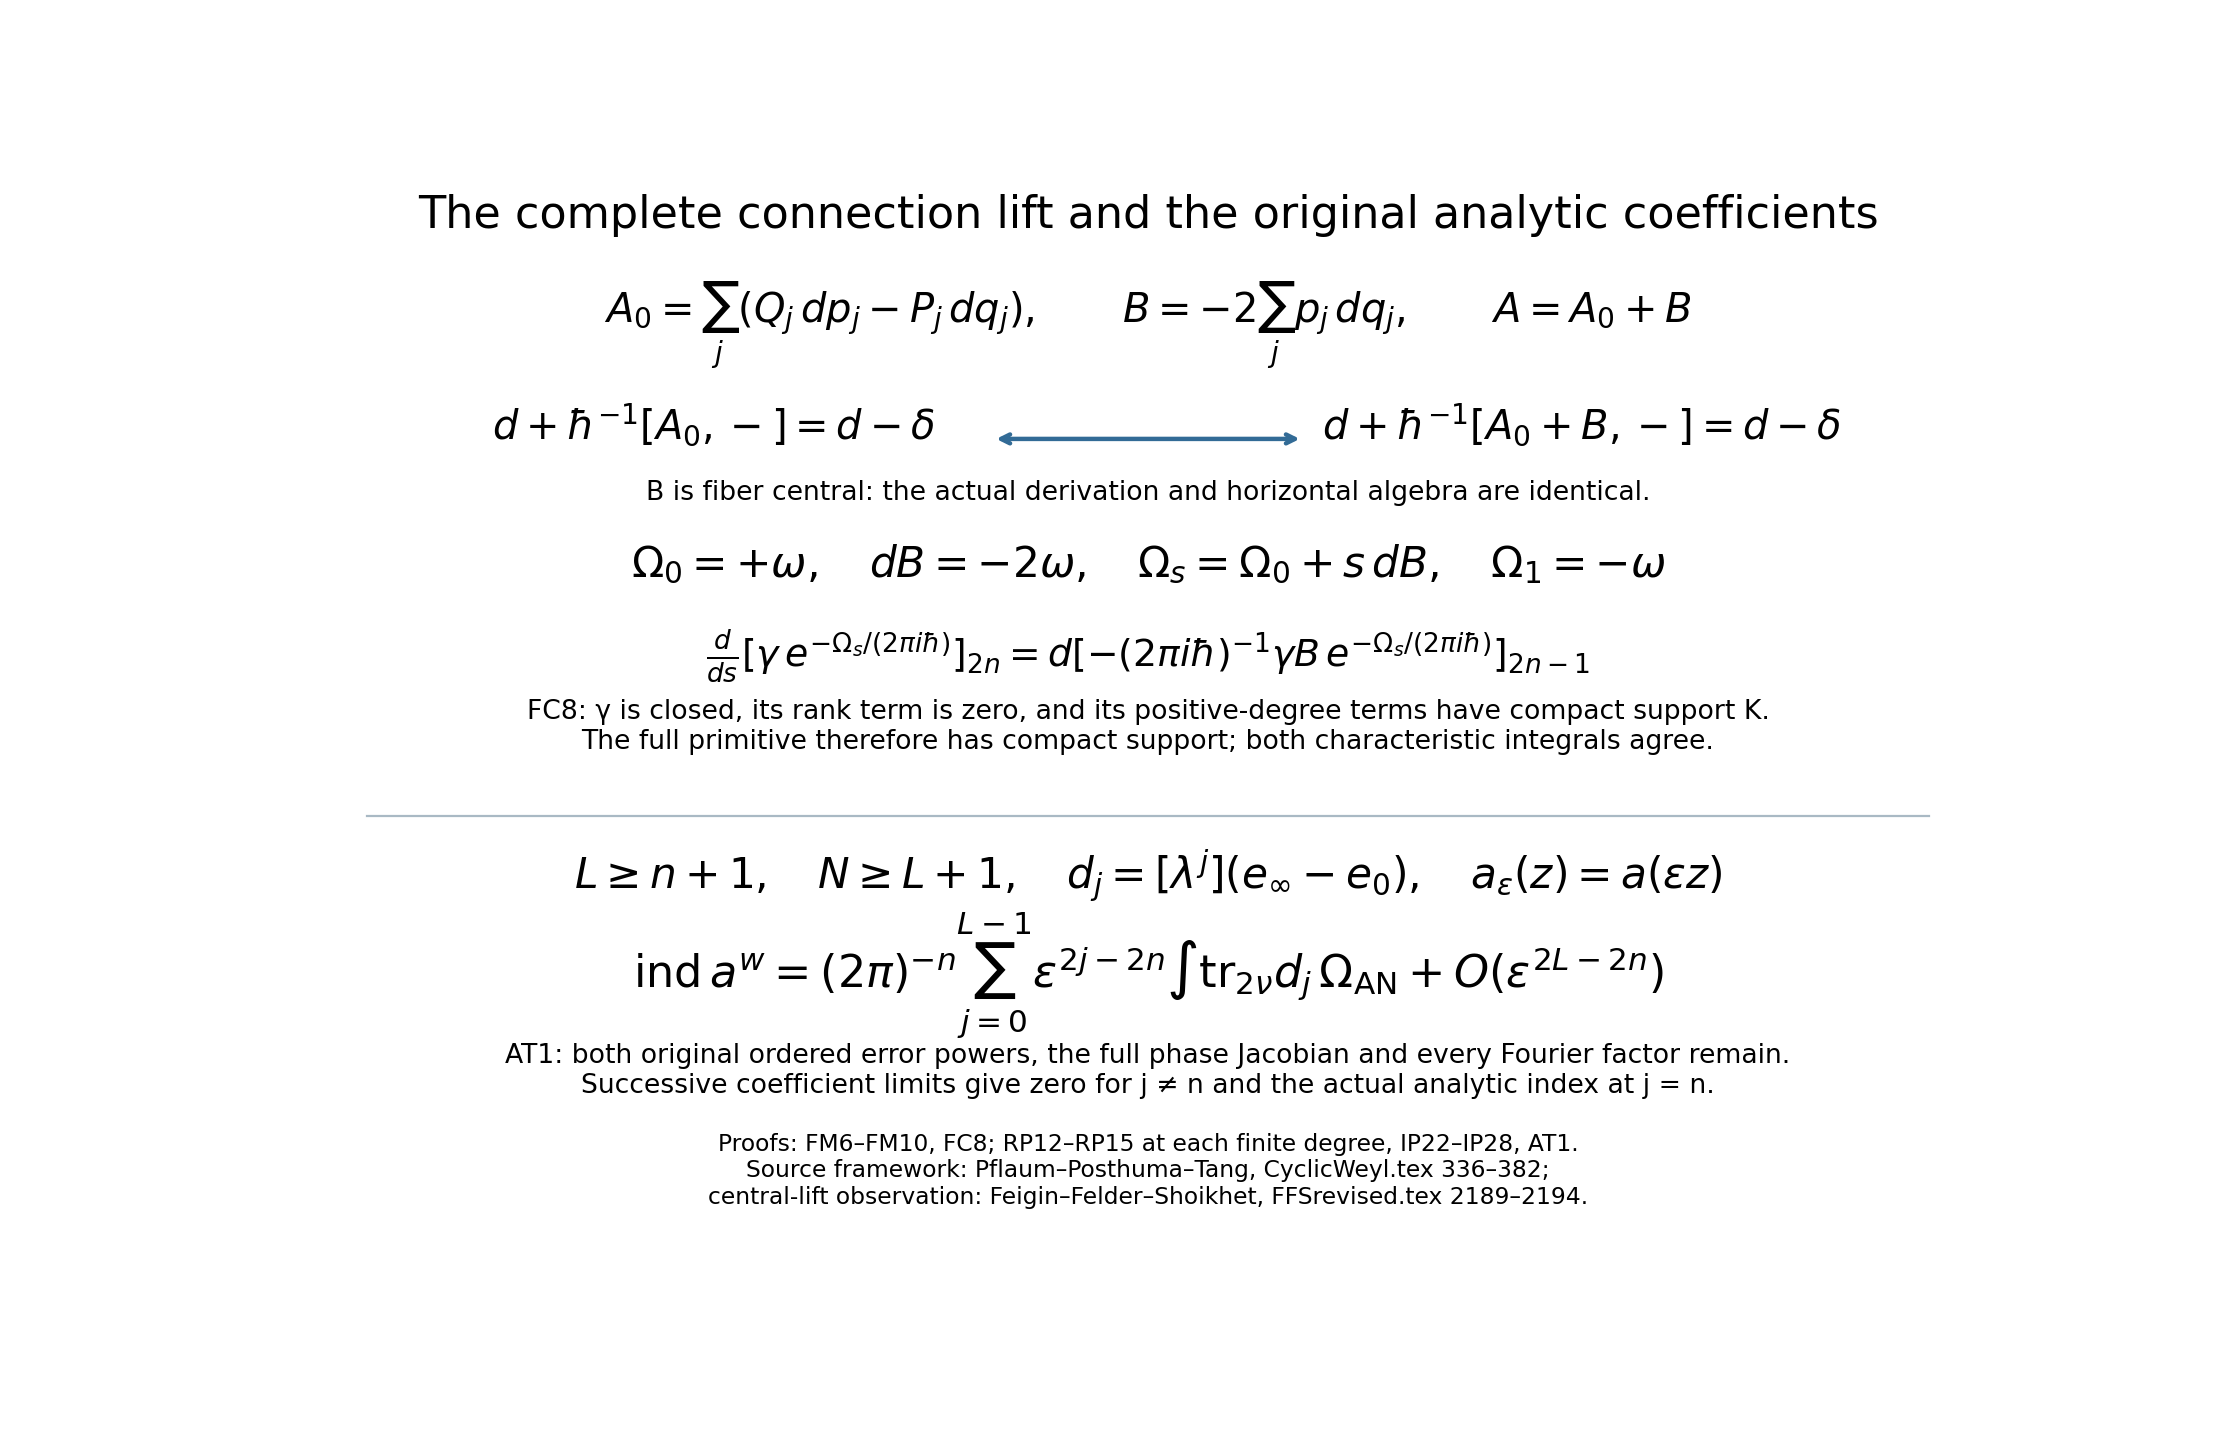
\includegraphics[keepaspectratio,alt={The full central connection change and the original analytic coefficient comparison}]{../figures/matrix-index-receiving-maps.png}}
\caption{The full central connection change and the original analytic
coefficient comparison}
\end{figure}

FM6--FM9 and FC8 prove the exact central connection and curvature maps
in the figure. RP12--RP15, IP22--IP28 and AT1 prove the displayed
analytic coefficient comparison, with every original cutoff, ordered
error power, Jacobian and Fourier factor retained. The source connection
framework is Pflaum--Posthuma--Tang, CyclicWeyl.tex lines 336--382; the
central-lift observation is Feigin--Felder--Shoikhet, FFSrevised.tex
lines 2189--2194.

The scaled Weyl lesson proves \(\operatorname{ind}a^w=A_n\), where
\(A_n\) is its complete finite ordered Weyl coefficient, including every
\(C_k\) and cutoff derivative. Equation (MB9) identifies its integrated
value with the original cutoff expression. This route uses the full
relative projector, exact source cyclic trace and source index theorem.
The independent direct proof is
\href{ordered-weyl-exterior-reduction.pdf}{From ordered Weyl errors to
the exterior index form}, equations (5)--(18): it proves the complete
multi-degree selection, atomic derivative involution, ordered exterior
count and full beta moment for every integer error power \(N>n\). Its
equation (17) is exactly the cutoff expression in (MB9); its equation
(18) gives the same outward boundary value in (MB10). The two complete
arguments therefore agree on the actual original operators.

\subsection{5. The product metric and left
quantization}\label{the-product-metric-and-left-quantization}

\subsubsection{5.1 Retain the original product
structure}\label{retain-the-original-product-structure}

Let \(n\ge1\) and keep the two coordinate groups \(z=(x,\xi)\),
\(x,\xi\in\mathbb R^n\), with the actual metrics \[
 G_z=\frac{|dx|^2}{\langle x\rangle^2}
       +\frac{|d\xi|^2}{\langle\xi\rangle^2},
 \qquad
 g_z=\frac{|dx|^2+|d\xi|^2}
           {1+|x|^2+|\xi|^2},
 \qquad
 \Omega_{\rm AN}=dx_1\wedge d\xi_1\wedge\cdots
                  \wedge dx_n\wedge d\xi_n .
 \tag{PM1}
\] Assume the full matrix symbol
\(a\in S(1,G;\operatorname{End}\mathbb C^\nu)\) has a uniformly bounded
inverse outside some ball \(B_{R_0}\). Choose the original \emph{cutoff
inverse} \(\chi\) with \(\chi=1\) for \(|z|\ge R_0\), supported in the
invertibility region, and write \(b=\chi a^{-1}\) there, extended by
zero. Then \(ba=ab=\chi I_\nu\), with the two matrix orders retained.
Let \(\partial B_R\), \(R>R_0\), have the outward orientation induced by
\(\Omega_{\rm AN}\). The \emph{radial profile} \(\psi_{\rm rad}\) below
is a different scalar function from \(\chi\).

Equations (RC3) and (RC9) construct, for every fixed sufficiently small
\(\varepsilon>0\), \[
 F_\varepsilon(z)=\psi_{\rm rad}(\varepsilon z)z,\qquad
 a_\varepsilon=a\circ F_\varepsilon\in S(1,g),\qquad
 F_\varepsilon(z)=z
   \quad\text{when }|\varepsilon z|\le1 .
 \tag{PM2}
\] For \(|\varepsilon z|\ge2\), \(F_\varepsilon(z)=z/(\varepsilon|z|)\),
so its image is on the sphere of radius \(1/\varepsilon\). Choose
\(1/\varepsilon>R_0\); then \(a_\varepsilon\) is uniformly invertible at
phase infinity with the same exterior inverse bound as \(a\), evaluated
on that sphere. This checks every hypothesis of MB1--MB10 for
\(a_\varepsilon\); it does not pretend that the endpoint \(a=a_0\) lies
in \(S(1,g)\).

\subsubsection{5.2 The fixed boundary and the analytic
endpoint}\label{the-fixed-boundary-and-the-analytic-endpoint}

Equations (PT2)--(PT9) construct both product-metric Weyl error sides
for \(a_\varepsilon\) and \(a_0=a\), with the exact common compact
cutoff defect \(1-\chi_\varepsilon=1-\chi\) for small \(\varepsilon\).
Taking \(N=2n+2\), Equation (PT7) supplies one integrable majorant for
every original weighted trace-class seminorm of both \(N\)-th error
powers. Equation (PT9) then proves trace-norm convergence of those
powers, and Equation (PT10) concludes \[
 \operatorname{ind}(a\circ F_\varepsilon)^w
   =\operatorname{ind}a^w
   \quad\text{for all sufficiently small }\varepsilon>0 .
 \tag{PM3}
\] This is an operator-index equality derived from the original full
errors, not a claim of operator-norm convergence of \(a_\varepsilon^w\).

After fixing \(R>R_0\), make \(\varepsilon\) smaller so that
\(\varepsilon R<1\). Then \(F_\varepsilon\) is the identity on a
neighborhood of \(\partial B_R\). Equation (PT11) gives both the exact
symbol and tangential one-form equalities there: \[
 a_\varepsilon|_{\partial B_R}=a|_{\partial B_R},
 \qquad
 (a_\varepsilon^{-1}da_\varepsilon)|_{T\partial B_R}
  =(a^{-1}da)|_{T\partial B_R}.
 \tag{PM4}
\] The sphere, its outward orientation and all \(2n-1\) matrix-valued
one-form factors are identical on the two sides. No global
change-of-variables factor is needed: the comparison occurs on the
\textbf{same fixed sphere}, where the radial map is literally the
identity.

Apply the proved isotropic theorem MB10 to \(a_\varepsilon\), then use
(PM3)--(PM4). The exact product-metric matrix Weyl index is \[
 \boxed{\quad
 \operatorname{ind}a^w
 =-(-2\pi i)^{-n}\frac{(n-1)!}{(2n-1)!}
   \int_{\partial B_R}^{\Omega_{\rm AN}}
       \operatorname{tr}_{\nu}
          [(a^{-1}da)^{2n-1}] .
 \quad}
 \tag{PM5}
\] The coefficient is MB10's original one, including its sign and both
factorials. The proof holds at every \(n\ge1\) and matrix rank \(\nu\)
under the stated product-metric hypotheses.

\subsubsection{5.3 The cutoff and left-quantization
versions}\label{the-cutoff-and-left-quantization-versions}

The same \(\chi\) in (PM1) gives \(b=\chi a^{-1}\) and the full original
compact differential form
\((1-\chi)^n\operatorname{tr}[(db\wedge da)^n]\). Equations (BN1)--(BN5)
derive its exact transgression and beta moment solely from this identity
on the invertibility region and compact cutoff support. Applying (BN5)
to the original \(a,b,\chi\), and comparing its written coefficient with
(PM5), gives the equivalent \textbf{product-metric cutoff formula} \[
 \boxed{\quad
 \operatorname{ind}a^w
 =(2\pi)^{-n}\frac{2}{i^n n!}
   \int_{\mathbb R^{2n}_{x,\xi}}^{\Omega_{\rm AN}}
       (1-\chi)^n
       \operatorname{tr}_{\nu}[(db\wedge da)^n].
 \quad}
 \tag{PM6}
\] The cutoff formula here is for the \emph{original} product symbol,
not for \(a_\varepsilon\); it follows from the original transgression
and the common boundary integral. Every coefficient is the same as MB9
and equation (17) of \href{ordered-weyl-exterior-reduction.pdf}{From
ordered Weyl errors to the exterior index form}.

Finally (PT12) is the exact left-to-Weyl symbol identity \[
 \operatorname{Op}_0(a)
  =\operatorname{Op}_{1/2}(a_{\rm W}),\qquad
 a_{\rm W}
   =\exp\!\left(-\frac{i}{2}
             \langle D_x,D_\xi\rangle\right)a,
 \qquad
 a_{\rm W}-a\in S(h_G,G),\quad
 h_G=\frac{1}{\langle x\rangle\langle\xi\rangle}.
 \tag{PM7}
\] The product Planck weight tends to zero at full phase infinity, so
the actual operator difference is compact by the metric operator bounds
lesson. Equation (PT14) proves equality of Fredholm indices. Equations
(PM5)--(PM6) therefore give \textbf{the same exact numerical values} for
the original left quantization: \[
 \boxed{\quad
 \operatorname{ind}\operatorname{Op}_0(a)
  =\operatorname{ind}a^w
  =-(-2\pi i)^{-n}\frac{(n-1)!}{(2n-1)!}
     \int_{\partial B_R}^{\Omega_{\rm AN}}
       \operatorname{tr}_{\nu}[(a^{-1}da)^{2n-1}] .
 \quad}
 \tag{PM8}
\]

The left and Weyl operators and their symbols remain distinct. Their
proved compact correction identifies their indices. The full finite
term-by-term integration is proved independently in
\href{ordered-weyl-exterior-reduction.pdf}{From ordered Weyl errors to
the exterior index form}, equations (5)--(18).

The metric assumptions set the scope of this result. The isotropic
metric is covered by the matrix-index argument, and the product metric
by the radial transport just proved. For a general \(\sigma\)-temperate
metric \(g\), let \(g^\sigma\) be its symplectic dual. The further
condition \(\sup_{v\ne0}g_z(v)/g_z^\sigma(v)\to0\) as \(|z|\to\infty\)
does not by itself enter either proof above. This broader metric setting
is not established by either proof above. No general-metric index
theorem is asserted in this lesson.

\subsection{6. Worked example: a nonzero scalar
index}\label{worked-example-a-nonzero-scalar-index}

In one phase plane take \[
 a(x,\xi)=\frac{x+i\xi}{\sqrt{1+x^2+\xi^2}},
 \qquad (x,\xi)\in\mathbb R^2 .
 \tag{MI1}
\] For every multiindex \(\alpha\), differentiating the numerator and
denominator gives \(\lvert\partial^\alpha a(z)\rvert
\le C_\alpha\langle z\rangle^{-|\alpha|}\); thus \(a\in S(1,g)\). Its
only zero is at the origin and \(\lvert a(z)\rvert=|z|/\sqrt{1+|z|^2}\)
is bounded below outside any fixed ball about the origin. On the
positively oriented circle \(z=Re^{i\vartheta}\), the radial denominator
is positive and \(a^{-1}da=i\,d\vartheta\). Formula (MB10) at \(n=1\)
has coefficient \(-(-2\pi i)^{-1}=1/(2\pi i)\). Therefore \[
 \operatorname{ind}a^w
 =\frac{1}{2\pi i}\int_{\partial B_R}a^{-1}da
 =\frac{1}{2\pi i}\int_0^{2\pi}i\,d\vartheta
 =1 .
 \tag{MI2}
\] The full bounded symbol, the outward orientation and the original
Weyl operator are used; no unbounded model is substituted.

\subsection{7. Exercises with solutions}\label{exercises-with-solutions}

\textbf{Exercise 1.} Evaluate the exact boundary coefficient in (MB10)
for \(n=2\), retaining its sign and factorials.

\textbf{Solution.} Since \((-2\pi i)^2=-4\pi^2\) and
\((n-1)!/(2n-1)!=1/6\), the coefficient is
\(-(-4\pi^2)^{-1}/6=1/(24\pi^2)\). This uses the original
\(dx_1\wedge d\xi_1\wedge dx_2\wedge d\xi_2\) orientation.

\textbf{Exercise 2.} Let \(e_\infty-e_0=\sum_{j\ge0}\lambda^j d_j\) as
in (MB11). Show what the full formal identity (MB7) says about
\(d_{n+2}\).

\textbf{Solution.} Its contribution to
\(\mathcal T_\lambda(e_\infty-e_0)\) is
\((2\pi)^{-n}\lambda^2\int\operatorname{tr}_{2\nu}d_{n+2}\). The right
side of (MB7) has no \(\lambda^2\) term, so the integral is zero. No
pointwise assertion about \(d_{n+2}\) follows.

\subsection{References}\label{references}

The external higher algebraic index theorem is M. Pflaum, H. Posthuma
and X. Tang, \href{https://arxiv.org/abs/0805.1411}{arXiv:0805.1411v3},
original IndThms.tex, theorem thm:higher-algind. Its top local
Riemann--Roch antecedent is B. Feigin, G. Felder and B. Shoikhet,
\href{https://arxiv.org/abs/math/0311303}{arXiv:math/0311303v2},
original FFSrevised.tex. These are cited source results; the
specialization, exact normalizations and original-operator receiving
argument are proved above. The direct term-by-term integration of the
separate finite Weyl coefficient is completed in the direct
exterior-reduction lesson, equations (5)--(18).

\subsection{8. Editorial completion: a full proof of the operative flat
pairing}\label{editorial-completion-a-full-proof-of-the-operative-flat-pairing}

The source statements, all formulas and their order above are retained.
In this lesson (MB3) is an operative assertion: a citation alone would
not prove (MB7)--(MB10). We now prove (MB3) for its exact written
projectors and every dimension by the finite original Weyl calculation.
This supplies the complete required theorem specialization within the
programme. The more general theorem on other symplectic manifolds and
higher closed sequences is not invoked to fill any step below.

\subsubsection{8.1. Full tensor definitions and the actual smooth
horizontal
algebra}\label{full-tensor-definitions-and-the-actual-smooth-horizontal-algebra}

The exponential denoted by \(\mathcal E\) in (WR9) is the complete
source expression \[
 \mathcal E(u)=
 \left.\prod_{0\le r<s\le2n}
       \exp\bigl(\hbar(u_r-u_s+\tfrac12)\alpha_{rs}\bigr)
                  \right|_{u_0=0},\qquad
 \Delta^{2n}=\{0\le u_1\le\cdots\le u_{2n}\le1\}.
 \tag{LP1}
\] Every pair, the \(1/2\), the full parameter and the slot order are
retained. Its scalar constant derivative operators commute; this permits
regrouping derivative operators without regrouping the matrix factors.
For matrix-valued slots, the map \(\mu_{2n}\) evaluates their fiber
arguments at zero and takes the ordinary trace of their product in the
original order. Its scalar version omits only that final trace. A fixed
formal coefficient contains finitely many input degrees and contraction
degrees, so these maps are defined for smooth base coefficients as
formal differential expressions.

For such a coefficient, the notation \(u(p+P,q+Q)\) in (FM7) means its
full formal Taylor jet \[
 \widehat u=
 \sum_{\alpha,\beta\in\mathbb N^n}
       {P^\alpha Q^\beta\over\alpha!\beta!}
             (\partial_p^\alpha\partial_q^\beta u)(p,q).
 \tag{LP2}
\] It asserts no convergence of a Taylor series of a smooth function.
The equations \(\partial_{P_j}\widehat u=\partial_{p_j}\widehat u\) and
\(\partial_{Q_j}\widehat u=\partial_{q_j}\widehat u\) follow by
reindexing the individual coefficients, including the factorials.
Conversely, these equations and the value at \(P=Q=0\) determine every
coefficient by induction in its total fiber degree. Thus the
horizontal-lift and evaluation maps are exact inverses. At every base
formal degree, the diagonal chain rule and each finite fiber contraction
give exactly (FM10). This proves the full smooth horizontal algebra and
the exact (FM4) map with inverse, fixed supports and both matrix orders.

The determinant in (WR9) differentiates each of its \(2n\) connection
slots once. The full commutative exterior computation (WR4)--(WR6)
proves the divided Pfaffian normalization (WR8): its coefficient of an
ordered basis wedge is the sum of the distinct-plane determinants, each
occurring once after the written division. Sorting the pair containing
the first slot gives the full recurrence (WR3). Its base is \(\Pi_0=1\),
\(\Pi_2=\alpha_{01}\). Hence induction matches the source recurrence at
every degree, rather than assuming an exterior-power convention. On the
actual \(A\) in (FM6), all its central contributions have zero fiber
derivative and each remaining derivative is precisely \(-dq_j\) or
\(dp_j\). Every determinant permutation therefore contributes the same
oriented volume term in (FD6). After that operation every nonzero slot
other than slot zero is fiber constant. Every positive term of each
factor of (LP1) differentiates one of those constant slots, and is zero.
There are no remaining exponential terms.

For completeness, the volume of \(0\le u_1\le\cdots\le u_d\le r\) is
\(r^d/d!\): it is one for \(d=0\), and integrating the
\((d-1)\)-dimensional volume \(v^{d-1}/(d-1)!\) over the final
coordinate \(0\le v\le r\) proves the formula inductively. Thus all
\((2n)!\) determinant terms cancel exactly the \(1/(2n)!\) simplex
volume, while the original \((-1)^n\hbar^n\) and \(\hbar^{-2n}\) remain.
This proves (WR12) and (WR13) for every finite matrix rank. At degree
zero the pairing is evaluation on the actual relative difference;
(NS2)--(NS4) have one summand with the complete \((2\pi i)^{-n}\)
factor. Its cyclicity can also be proved here without a higher cocycle
theorem: (WR13) is the constant multiple of the compact coefficient
integral, and integration by parts annihilates every positive \(C_k\) by
antisymmetry of \(J\) against symmetric second derivatives, as proved in
FC1--FC3 of \href{relative-projectors-chern-cutoff.pdf}{the
relative-projector lesson}. Thus its degree-zero trace and pairing have
their actual domains and do not require an unproved general
cyclic-cohomology assertion.

\subsubsection{8.2. The full finite coefficient and every linear-path
hypothesis}\label{the-full-finite-coefficient-and-every-linear-path-hypothesis}

Fix an integer \(N>n\) and retain the original \(a,b,t=1-\psi\). Put
\(r_1=I-b\#_\lambda a\), \(r_2=I-a\#_\lambda b\), with their full formal
expansions. DE3--DE5 and OC27--OC30 of
\href{scaled-weyl-index-degree.pdf}{the scaled Weyl lesson} construct the
finite degree-\(n\) coefficient of \(r_1^{\#N}-r_2^{\#N}\), with every
intrinsic term and every later contraction. Both scaled analytic
remainders lie in the original \(S(h_\varepsilon^{n+1},g_\varepsilon)\),
with the complete product weight \((1+h_\varepsilon/4)^{4n}\) and its
derivative comparison in RP1--RP5. RA1--RA10 prove their actual
trace-norm bound \(C\varepsilon^2\). Each retained coefficient is
compact: in any degree at most \(n<N\), one of the \(N\) intrinsic slots
has degree zero, and its differentiated \(tI_\nu\) is supported in the
original \(K\). CI12 gives its trace with
\((2\pi)^{-n}\varepsilon^{-2n}\). T28 and IP16 give the index of the
unchanged \(a^w\) at every positive scale. The finite asymptotic
coefficient comparison consequently proves \[
 \operatorname{ind}a^w=(2\pi)^{-n}
       \int_{\mathbb R^{2n}}\operatorname{tr}_\nu
            [\lambda^n](r_1^{\#N}-r_2^{\#N})(z)\,dz.
 \tag{LP3}
\] To check that comparison directly, multiply the finite expansion by
\(\varepsilon^{2n}\) and take its limit to prove the degree-zero
coefficient zero; after each lower coefficient is zero, multiply by the
power which makes the next coefficient constant and take its limit. At
degree \(n\) the remainder tends to zero and gives (LP3). The whole
calculation is finite and has a proved trace-norm remainder.

We will use arbitrary invertible real linear maps only through their
exact original symbols. On a compact parameter interval let \(L_s\) be a
continuously differentiable path of invertible matrices, with
\(\|L_s\|\le C\), \(\|L_s^{-1}\|\le C'\). Then \[
 c\langle z\rangle\le\langle L_sz\rangle\le C''\langle z\rangle,
 \qquad
 \|\partial^\gamma(a\circ L_s)(z)\|
       \le C_\gamma\langle z\rangle^{-|\gamma|}.
 \tag{LP4}
\] The lower bound follows from \(|L_sz|\ge\|L_s^{-1}\|^{-1}|z|\),
retaining the term one in both brackets; the upper bound follows from
the operator norm. The chain rule gives the second inequality as the
complete finite sum of products of entries of \(L_s\) times the
corresponding derivative of the unchanged \(a\) at \(L_sz\). For its
parameter derivative differentiate that same sum. A derivative falling
on a matrix entry retains the same weight. A derivative falling on
\(a(L_sz)\) inserts \(\dot L_sz\), bounded by \(C|z|\), and one further
derivative of \(a\), with weight \(\langle L_sz\rangle^{-|\gamma|-1}\);
the extra \(|z|\) leaves exactly the weight in (LP4). Integrating this
bound in \(s\) proves continuity of every original symbol seminorm. B26
proves operator-norm continuity. Exterior invertibility is preserved
because \(L_s^{-1}\) is uniformly bounded, and the original bounded
inverse evaluates at \(L_sz\). The corresponding cutoff is
\(\psi\circ L_s\), supported in the actual transformed inverse region,
with a fixed compact support for its defect along this compact path. The
full parametrix proves Fredholmness at every \(s\), so F6--F7 make the
index constant along the path. No assertion about a non-symplectic Weyl
algebra automorphism has been made.

Expand the integrand in (LP3) completely into occurrences of the
original atomic factors \(a,b,t\). Each term has exactly \(2n\) labeled
coordinate derivatives. Let \(I_\alpha\) be the integral of the entire
group with counts \(\alpha_j\) in each original coordinate, including
all its scalar coefficients and ordered matrix words, where
\(|\alpha|=2n\). Positive diagonal maps \(D_\rho\) are joined to the
identity by their positive diagonal path; (LP4) proves every hypothesis
of the preceding index argument. Each derivative supplies its
\(\rho_j\), while the actual positive Jacobian is \(\prod_j\rho_j\).
Hence \[
 \operatorname{ind}a^w=(2\pi)^{-n}
   \sum_{|\alpha|=2n}I_\alpha
               \prod_{j=1}^{2n}\rho_j^{\alpha_j-1}
       \quad(\rho_1,\ldots,\rho_{2n}>0).
 \tag{LP5}
\] This is a finite Laurent identity. Here is its complete independence
argument. Include the exponent zero in its finite exponent set, and
choose an integer vector \(v\) with pairwise distinct dot products on
that set. Such a vector exists: \(v=(1,m,\ldots,m^{2n-1})\) fails a
prescribed distinct pair only when the integer \(m\) is a root of its
nonzero difference polynomial. Each such polynomial has finitely many
roots by induction on its degree using polynomial division at a root,
and there are finitely many pairs. Choose an integer outside their
union. Substitution \(\rho_j=e^{s v_j}\) gives a finite exponential
identity. Differentiating it at \(s=0\) through one less than the number
of exponents gives its Vandermonde system. The determinant is
\(\prod_{r<t}(c_t-c_r)\ne0\): subtracting two equal columns at
\(c_r=c_t\) shows all these factors divide the determinant, and its
highest-degree term fixes their coefficient to one. Thus the distinct
coefficients are zero. Consequently \[
 I_\alpha=0\quad(\alpha\ne\mathbf1),\qquad
 \operatorname{ind}a^w=(2\pi)^{-n}I_{\mathbf1}.
 \tag{LP6}
\]

A reflection in one original coordinate multiplies the unique surviving
derivative-count group by minus one; its absolute Jacobian is one.
Applying (LP3)--(LP6) to that reflected symbol proves its index is the
negative of the original. Every positive-determinant invertible matrix
is joined to the identity by a path as in (LP4). To prove this last
statement, Gram--Schmidt factors it into an orthogonal matrix and an
upper triangular matrix with positive diagonal. Linear interpolation of
the latter to its diagonal and then of its diagonal to the identity
keeps every diagonal positive. An orthogonal matrix of determinant one
is reduced to the identity by coordinate-plane rotations. For two
entries \(a,b\) in slots \(1,j\), if \(r=\sqrt{a^2+b^2}>0\), the
rotation with matrix \(\begin{pmatrix}a/r&b/r\\-b/r&a/r\end{pmatrix}\)
sends them to \((r,0)\); if both entries are zero, leave them unchanged.
Applying this successively for \(j=2,\ldots,2n\) sends its first unit
column to the first basis vector. Repeat on the orthogonal complement.
The last one-dimensional orthogonal factor is one because the
determinant remains one. Every rotation has its sine/cosine path from
the identity, including the half-turn when \(a<0,b=0\). The resulting
finite paths remain invertible on compact intervals, so the bounds in
(LP4) hold. For a coordinate permutation, its sign is therefore its
index transport sign. This proves the complete alternation step in all
dimensions.

\subsubsection{8.3. The atomic involution, the surviving words, and the
full
count}\label{the-atomic-involution-the-surviving-words-and-the-full-count}

Let \(S^1\) be the original untraced differential expression with each
coordinate count one, so that \(I_{\mathbf1}=\int\operatorname{tr}S^1\).
For each coordinate-label permutation \(\sigma\), apply (LP6) to
\(a\circ P_\sigma\) and change back to the unchanged integration
variables. Its sign from the preceding paragraph is
\(\operatorname{sgn}\sigma\). Thus each integral of
\(\operatorname{sgn}\sigma\,S^1_\sigma\) equals \(I_{\mathbf1}\), and \[
 \operatorname{ind}a^w={ (2\pi)^{-n}\over(2n)!}
       \int\operatorname{tr} S^2\,dz,
 \qquad S^2=\sum_{\sigma\in S_{2n}}
                  \operatorname{sgn}\sigma\,S^1_\sigma.
 \tag{LP7}
\] In each fully expanded atomic word, if two derivative slots reach the
same occurrence of \(a,b\) or \(t\), transpose their coordinate labels.
The unchanged mixed derivatives commute on that occurrence; all other
slots and every matrix position remain unchanged. The transposition
reverses the alternating sign and has no fixed point because the labels
are distinct. Pairing all permutations by this involution cancels that
entire word. This is a finite sum of pairs, not an assumed matrix
cancellation.

For completeness, every later contraction of an ordered \(N\)-fold
product is generated by the finite degree part of \[
 \left.\exp\left({\lambda\over2i}
       \sum_{1\le r<s\le N}\sum_{u,v}J^{uv}
                \partial_{z_{r,u}}\partial_{z_{s,v}}\right)
               \prod_{r=1}^N f_r(z_r)\right|_{z_1=\cdots=z_N=z}.
 \tag{LP8}
\] Its coefficients follow by induction from the diagonal chain rule:
contracting a product of the first slots against the next slot is the
sum of their pair contractions. These scalar operators commute, so the
finite multinomial formula gives the displayed exponential coefficients,
with their original factorials. Matrix factors keep their order
throughout. Any intrinsic \(C_k(b,a)\) or \(C_k(a,b)\) with \(k\ge2\)
has two derivatives on each of its two atomic occurrences, and cancels
by the involution. Any later contraction reaching a first intrinsic
bracket likewise makes one of its atomic occurrences carry a second
derivative, and cancels. Among remaining scalar \(t\)-occurrences, the
contraction graph has degree at most one at every vertex, and hence is a
matching. Each of its edges is the exact scalar factor
\(\sum_j(t_{\xi_j}t_{x_j}-t_{x_j}t_{\xi_j})=0\). The scalar factors can
be moved past the other factors without moving any matrix factor; that
whole edge contribution is zero. These cases exhaust every contraction
in (LP8).

Only undifferentiated scalar \(t\)'s and first intrinsic brackets
remain. Since \(-C_1(b,a)=(i/2)\{b,a\}\), their full expression before
taking the alternating sum is \[
 \binom Nn t^{N-n}\left({i\over2}\right)^n
            \bigl(\{b,a\}^n-\{a,b\}^n\bigr),
 \qquad
 \{b,a\}=\sum_j(b_{\xi_j}a_{x_j}-b_{x_j}a_{\xi_j}).
 \tag{LP9}
\] Exactly \(n\) of the \(N\) original error slots supply a bracket,
accounting for the full binomial. The two matrix brackets have not been
replaced by negatives of one another.

Put
\(\widetilde\Omega=d\xi_1\wedge dx_1\wedge\cdots\wedge d\xi_n\wedge dx_n=(-1)^n\Omega_{\rm AN}\).
A bracket word using each coordinate once uses each canonical pair once.
It has \(n!\) choices of the order of pairs and \(2^n\) choices of their
internal bracket terms. For any fixed ordered exterior word in
\((db\wedge da)^n\), every one of these \(2^n n!\) base words has one
unique coordinate-label permutation taking it to the target word. The
base bracket sign times that permutation sign is precisely the target
exterior sign: an internal pair switch contributes one minus, and a
switch of two length-two blocks contributes plus. Thus every exterior
word occurs with exactly the same multiplicity. The original factor
\((i/2)^n\) leaves \(n!i^n\), proving the untraced identity \[
 S^2\widetilde\Omega=n!i^n\binom Nn t^{N-n}
       \bigl((db\wedge da)^n-(da\wedge db)^n\bigr).
 \tag{LP10}
\] The finite graded matrix trace is proved entry by entry in ES1 of the
relative-projector lesson. Moving the first one-form past the other
\(2n-1\) one-forms gives
\(\operatorname{tr}(da\wedge db)^n=-\operatorname{tr}(db\wedge da)^n\).
Inserting (LP10) in (LP7), with the pair-order sign and every factorial
retained, gives \[
 \operatorname{ind}a^w=(2\pi)^{-n}
     {2\,n!\over i^n(2n)!}\binom Nn
       \int^{\Omega_{\rm AN}}t^{N-n}
                           \operatorname{tr}_\nu[(db\wedge da)^n].
 \tag{LP11}
\] The numerator is twice \(n!\), and the denominator retains \((2n)!\).
Choosing \(N=2n>n\) retains \(t^n\) and the exact factor
\(\binom{2n}{n}\), so \[
 \operatorname{ind}a^w=(2\pi)^{-n}{2\over i^n n!}
       \int^{\Omega_{\rm AN}}(1-\psi)^n
                           \operatorname{tr}_\nu[(db\wedge da)^n].
 \tag{LP12}
\] This proves (MB9) directly at its entire original scope. Every finite
original Weyl term was either retained in (LP9) or paired by an explicit
zero mechanism before this integration. Sections2--6 of
\href{ordered-weyl-exterior-reduction.pdf}{the direct exterior-reduction
lesson} record the same calculation; the detailed proof above supplies
its use within the present lesson without importing an external index
theorem.

\subsubsection{8.4. The exact two sides of MB3, including the full
curvature}\label{the-exact-two-sides-of-mb3-including-the-full-curvature}

The relative-projector lesson's FC5--FC11 prove, by arbitrarily deep
finite expansions and actual trace-norm remainders, \[
 \mathcal T_\lambda(e_\infty-e_0)
       =(2\pi\lambda)^{-n}\tau_{2\nu}(e_\infty-e_0)
       =\operatorname{ind}a^w.
 \tag{LP13}
\] Its complete proof is also the finite argument already written in
(AT1): for each prescribed coefficient choose a fixed deeper integer
truncation before sending \(\varepsilon\) to zero. It does not assign
convergence to a formal series. Combining the actual flat density
(WR14), (LP13) and (LP12) gives its entire source pairing value
\((-1)^n\) times the right side of (LP12).

Here are all characteristic-side prerequisites with no imported theorem.
The global conjugating matrix \(U_0\) supplies a smooth frame for
\(V_P\) from its first \(\nu\) columns and a complementary frame from
its other columns, so both the image and kernel of the actual
nonorthogonal \(P\) are smooth bundles. The original Grassmann operator
\(P\,d\) obeys the connection product rule; its full curvature
calculation is (CN4). Differentiating \(P^2=P\) makes \(dP\)
off-diagonal, so \((dP)^2\) commutes with \(P\). This proves (CN5), and
the finite trace of every odd power is zero by that block decomposition.
Thus all the closed relative forms in (FC3) are globally defined and
compact; their degree-zero rank difference is identically zero. The
chosen tangent connection has zero curvature, so the complete formal
series \(\det[(Y/2)/\sinh(Y/2)]^{1/2}\) has value one at \(Y=0\), its
constant term. No statement about a nonflat characteristic class is
needed.

The tangent connection choice also has a complete local comparison. Any
other smooth connection on this globally trivial tangent bundle has a
matrix one-form \(C\). Put \(C_s=sC\) and \(R_s=dC_s+C_s\wedge C_s\).
Direct expansion proves \(d_{C_s}R_s=0\) and \(\partial_sR_s=d_{C_s}C\),
where \(d_{C_s}v=dv+C_s\wedge v-(-1)^{\deg v}v\wedge C_s\). The full
graded matrix trace therefore gives \(d\operatorname{tr}R_s^j=0\) and
\(\partial_s\operatorname{tr}R_s^j=j\,d\operatorname{tr}(C\wedge R_s^{j-1})\),
for every \(j\ge1\), with no reordered matrix products. At each exterior
degree the written characteristic series
\(\det[(R_s/2)/\sinh(R_s/2)]^{1/2}\) is a finite polynomial in these
traces. Indeed the formal identity
\(\det f(Y)^{1/2}=\exp[\tfrac12\operatorname{tr}\log f(Y)]\), with
\(f(Y)=(Y/2)/\sinh(Y/2)\) and constant term one, follows by the adjugate
differentiation formula for the determinant, its inverse geometric
series, and equality of the initial constant terms; comparison of
successive formal coefficients proves the identity. Thus each
positive-degree derivative of the characteristic form is exact: apply
the displayed trace derivative to one factor of each finite polynomial
and retain the other closed factors. Integrating in \(s\) gives
\(\hat A(C)-1=d\eta_C\) with the full characteristic coefficients
retained. The product of \(\eta_C\) with the original closed
\(\gamma\wedge e^{-\Omega_F/(2\pi i\hbar)}\) is compact. The proved
compact Stokes receiver consequently shows that this actual connection
change leaves the entire relative characteristic integral unchanged
coefficient by coefficient. This establishes the connection-choice
assertion in Section3 without invoking a general characteristic-class
theorem.

The radial primitive (FC5) also has an exact coordinate proof. Write
\(\beta_{ij}=-\beta_{ji}\) for a closed two-form and
\((H\beta)_j=\sum_l z_l\int_0^1s\beta_{lj}(sz)\,ds\). Differentiating
under this compact parameter integral and using the full closedness
identity gives \[
 \begin{aligned}
 (dH\beta)_{ij}
 &=\int_0^1\left[2s\beta_{ij}(sz)
       +s^2\sum_lz_l\partial_l\beta_{ij}(sz)\right]ds\\
 &=\int_0^1{d\over ds}\bigl(s^2\beta_{ij}(sz)\bigr)ds
   =\beta_{ij}(z).
 \end{aligned}
 \tag{LP14}
\] The endpoint at zero is zero by smoothness. Hence every original
formal coefficient of \(\Omega_F\) has its written global primitive. In
top degree, the full exponential in (CN1) is a finite sum of exterior
powers; a prescribed Laurent coefficient of it is a finite sum as well
because its exterior power is bounded by \(n\) and the curvature has no
negative intrinsic formal powers. Each term with a positive curvature
power has exactly the compact primitive (FC6), including its factorial,
power of \(2\pi i\) and negative parameter powers. ES5--ES7 of the
relative-projector lesson prove the required full-space and ball Stokes
receivers in the actual original orientation. Their integral is
therefore zero; no curvature contribution was suppressed before this
exact comparison.

The surviving characteristic term is the full Grassmann top form
\(1/[n!(2\pi i)^n]\operatorname{tr}P(dP)^{2n}\). The original compact
exact defect (CP11)--(CP14), with its full polynomial and both
endpoints, proves its integral equals the right side of (LP12). The
source oriented coordinate swap supplies the single \((-1)^n\) in (CN7).
Thus its characteristic value is also \((-1)^n\) times that same right
side. We have proved both sides of (MB3) equal, on its exact actual
pair, all matrices and all dimensions. This proves (MB3), (MB7), (MB9)
and their formal and analytic receiving maps without assuming the higher
algebraic index theorem or local Riemann--Roch theorem. Their cited
general formulations remain free reference context; they are not missing
proof prerequisites for these original programme conclusions.

\subsection{9. Editorial strengthening: every central formal lift and
every invertible linear
map}\label{editorial-strengthening-every-central-formal-lift-and-every-invertible-linear-map}

\subsubsection{9.1. Arbitrary higher curvature terms are actually
realized}\label{arbitrary-higher-curvature-terms-are-actually-realized}

Keep the same unchanged flat horizontal algebra, and let \(\beta_j\) be
any closed smooth scalar two-forms for \(j\ge1\). Define the full
central one-form and curvature \[
 B_\beta=-2\sum_jp_jdq_j+
           \sum_{r\ge1}\hbar^r H\beta_r,
 \qquad A_\beta=A_0+B_\beta,
 \qquad \Omega_\beta=-\omega+\sum_{r\ge1}\hbar^r\beta_r.
 \tag{CL1}
\] The commutator with a central scalar one-form is zero as a derivation
of sections, so (FM7) and the horizontal jets (LP2) are unchanged. Its
graded self-commutator and cross commutators are zero because exterior
scalar one-forms anticommute and scalar coefficients commute. The full
curvature is therefore
\(dB_\beta+\hbar^{-1}A_0\wedge_\star A_0=-\omega+\sum\hbar^r\beta_r\),
by (FM8) and (LP14). This proves an actual connection realizing every
written higher coefficient, rather than merely an exactness assertion
about a prospective curvature.

Every term of the determinant density containing any slot from
\(B_\beta\) is zero after that slot's fiber derivative. Thus the full
density and its degree-zero pairing are identical coefficient by
coefficient for all these lifts. On the characteristic side, the full
transgression (FC8) with \(B_\beta-B\) has compact primitive, retaining
all exponential factors and inverse powers; equivalently (FC6) proves
all positive curvature terms integrate to zero. Hence the completely
proved equality (MB3) holds for the exact same relative pair under every
lift (CL1). The identity map on horizontal sections, the identical
algebra product, the unchanged compact support and the explicit central
curvature morphism are all proved. No general existence theorem for
nonflat Fedosov connections is being used.

\subsubsection{9.2. Linear index transport and the exact algebra
defect}\label{linear-index-transport-and-the-exact-algebra-defect}

Let \(L\in GL(2n,\mathbb R)\), preserve \(a_L=a\circ L\),
\(b_L=b\circ L\), \(\psi_L=\psi\circ L\), and \(K_L=L^{-1}K\). The exact
path proof (LP4) and its reflection computation give the stronger index
comparison \[
 \operatorname{ind}(a\circ L)^w
       =\operatorname{sgn}(\det L)\operatorname{ind}a^w.
 \tag{LI1}
\] For negative determinant, compose with one fixed coordinate
reflection to obtain positive determinant, apply its proven path and
then the negative sign. All transformed original symbols remain in the
same isotropic class with their own exact finite bounds; no quantization
identity for a general linear change was presumed. Applying (LP13) to
each rebuilt original relative projector gives the corresponding exact
integrated formal trace with that same sign. This is index transport
between the actual bounded operators, not equality of their kernels.

There is also a full algebra map, with its exact failure object in the
original product. Write \(J_L=LJL^T\), retain all original ordered
derivatives, and define \(\#^{J_L}_\lambda\) by the complete formula
(RP7) with this displayed tensor. The chain rule proves at every
coefficient \[
 (f\circ L)\#^J_\lambda(g\circ L)
       =(f\#^{J_L}_\lambda g)\circ L.
 \tag{LI2}
\] This defines an exact algebra isomorphism from the smooth formal
algebra with tensor \(J_L\) to that with tensor \(J\), with inverse
pullback by \(L^{-1}\); supports map exactly by \(L^{-1}\), and matrices
retain their order. In the unchanged original \(J\)-product its defect
is the fully specified bilinear map \[
 \begin{aligned}
 \mathcal D_L(f,g)
 &:=(f\circ L)\#^J_\lambda(g\circ L)
                     -(f\#^J_\lambda g)\circ L\\
 &=\sum_{k\ge1}{\lambda^k\over(2i)^k k!}
   \left[\prod_{r=1}^k(J_L)^{u_rv_r}
                    -\prod_{r=1}^kJ^{u_rv_r}\right]
   \left[(\partial_{u_1}\cdots\partial_{u_k}f)
         (\partial_{v_1}\cdots\partial_{v_k}g)\right]\circ L.
 \end{aligned}
 \tag{LI3}
\] For formal input series the displayed contraction is further summed
over their finite intrinsic degrees, as in (RP7). Thus the nonzero
defect defines an exact family of deformed algebra structures and the
actual morphism (LI2); it is not an assertion of unrelated objects. If
\(J_L=J\), the defect is zero at every order. If \(J_L=-J\), the same
full comparison is the parameter map \(\lambda\mapsto-\lambda\),
retaining its \((-1)^k\) in every degree. A nonsymplectic index
comparison (LI1) therefore does not silently replace a product map by a
coordinate-only automorphism.

\begin{figure}
\centering
\pandocbounded{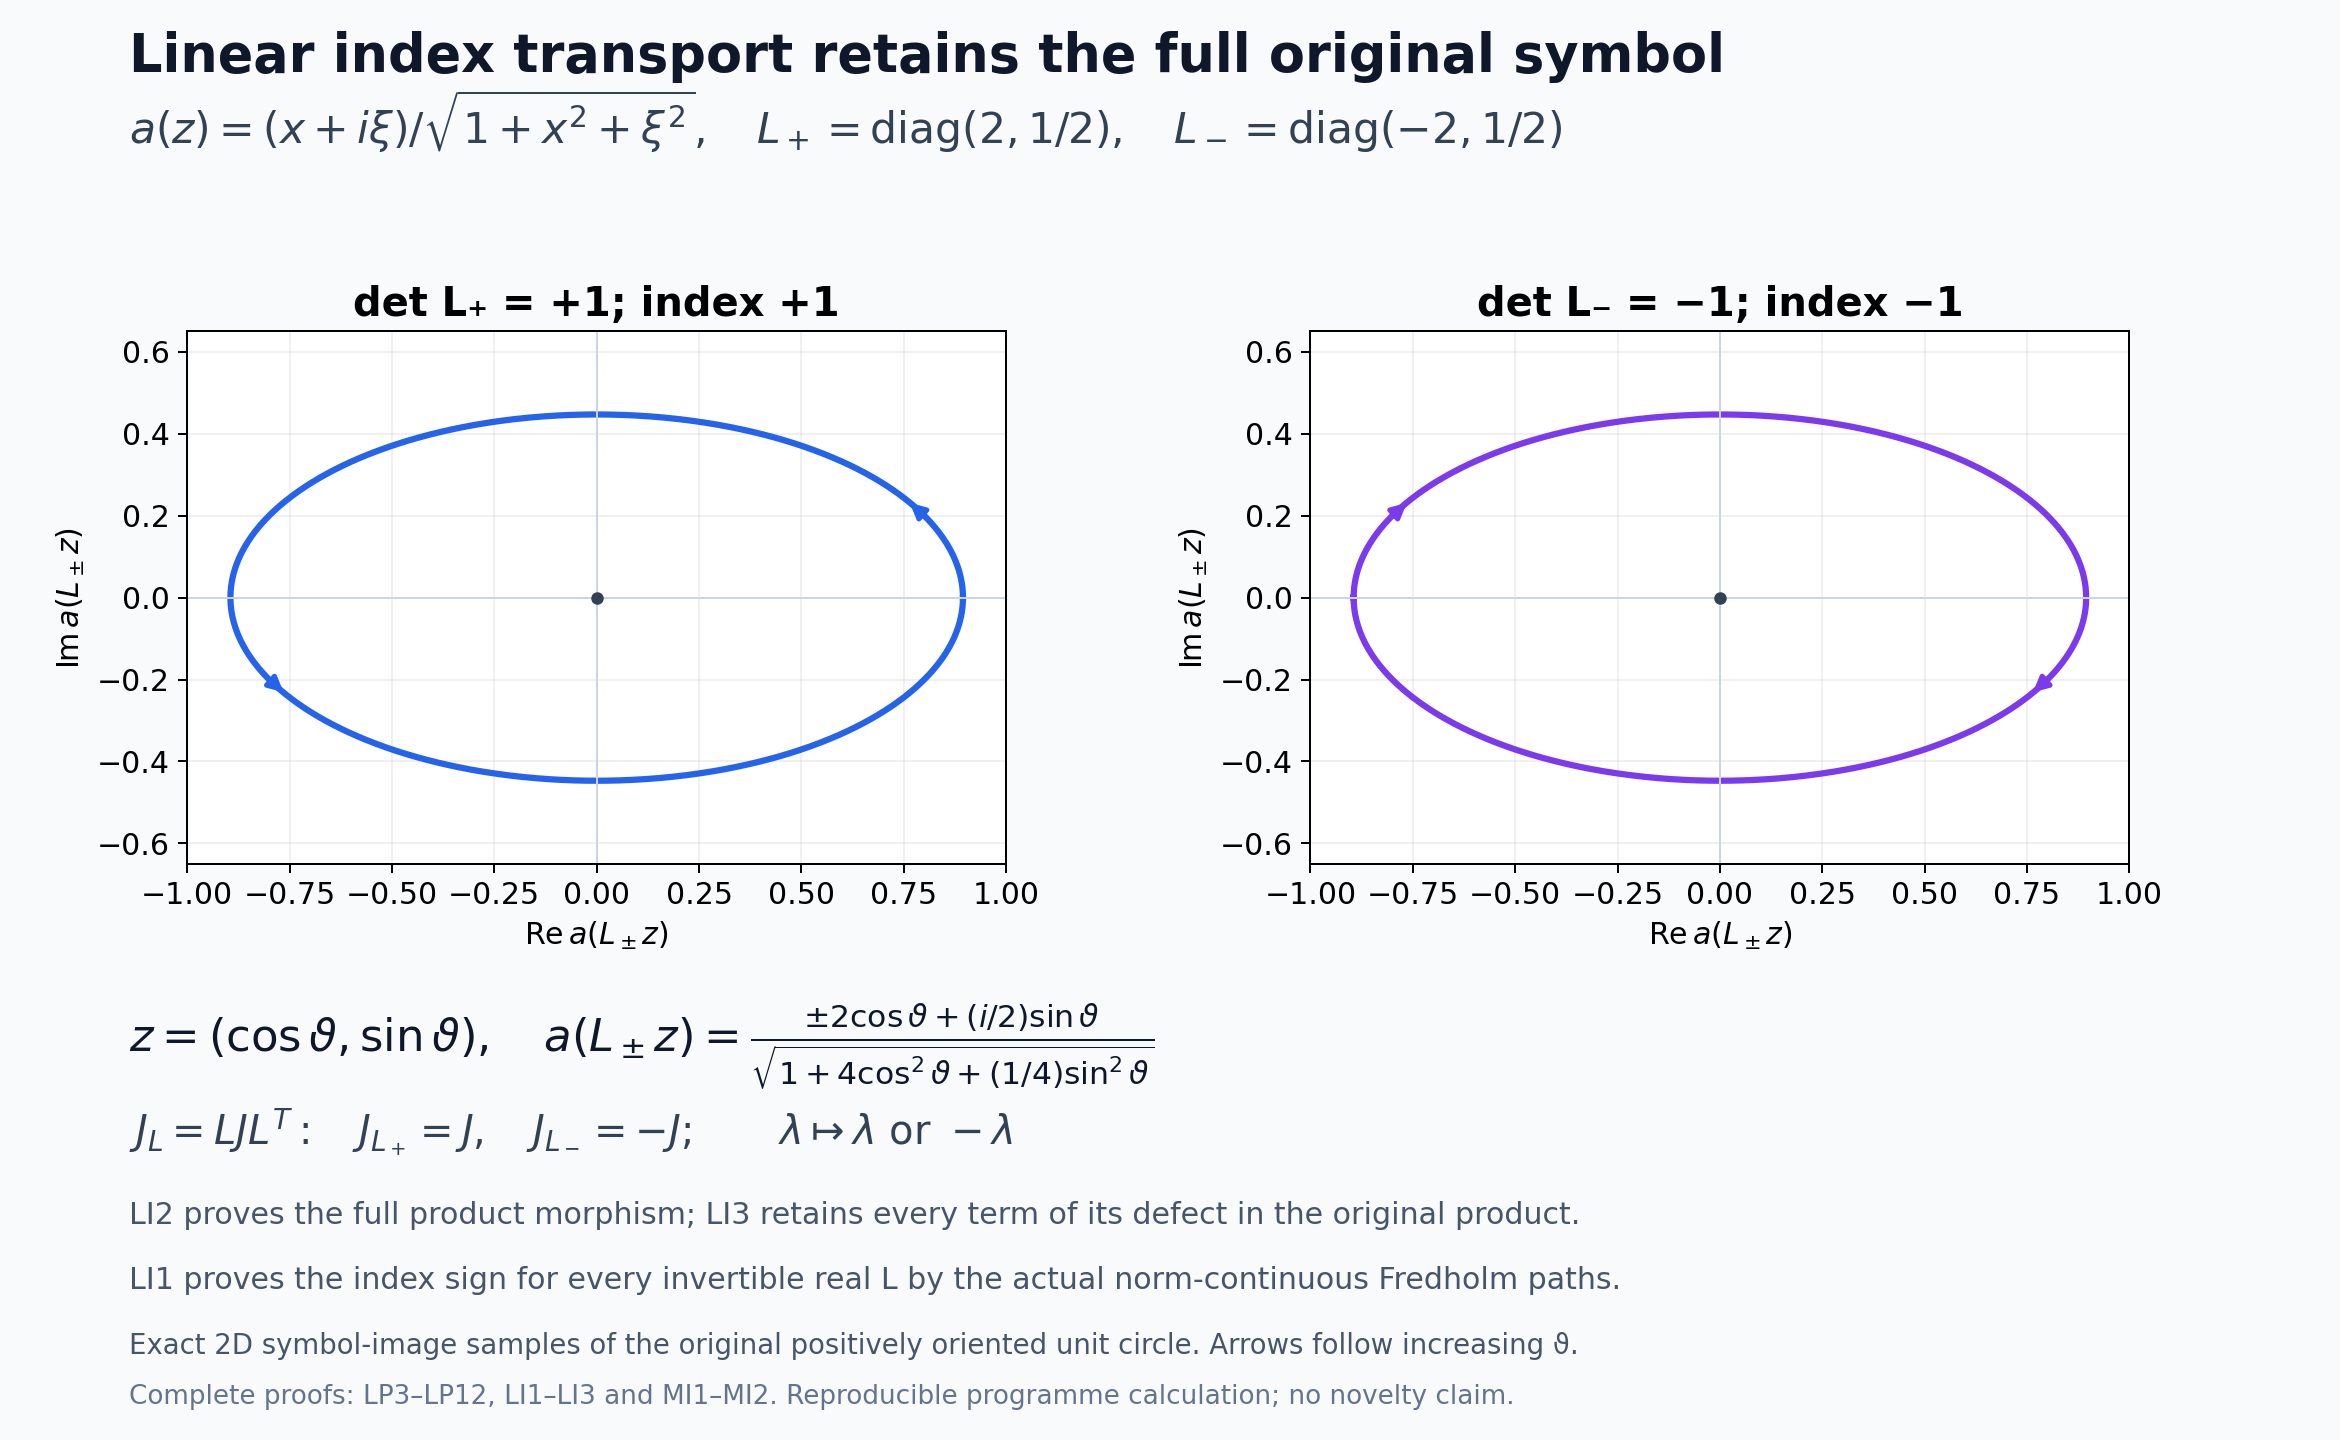
\includegraphics[keepaspectratio,alt={Exact linear pullbacks of the original bounded one-plane symbol}]{../figures/matrix-index-linear-maps.png}}
\caption{Exact linear pullbacks of the original bounded one-plane
symbol}
\end{figure}

These are exact two-dimensional symbol images of the original positively
oriented unit circle under the full MI1 symbol composed with
\(L_+=\operatorname{diag}(2,1/2)\) and
\(L_-=\operatorname{diag}(-2,1/2)\). The complete denominator remains
displayed; the arrows follow increasing circle parameter. LI1 proves the
respective original bounded Weyl indices \(+1\) and \(-1\). LI2--LI3
prove the exact tensor and parameter comparisons, rather than infer them
from the pictures. The
\href{../figures/matrix-index-linear-maps.py}{reproducible figure
source} accompanies the full proof.

\subsection{10. Editorial proof of the product endpoint and the original
example}\label{editorial-proof-of-the-product-endpoint-and-the-original-example}

\subsubsection{10.1. Every operative endpoint bound and both
quantizations}\label{every-operative-endpoint-bound-and-both-quantizations}

For (PM1)--(PM8), use the exact radial profile and separate cutoff
already defined there. RC4--RC7 of
\href{radial-symbol-index-transport.pdf}{the radial transport lesson}
prove all separate-coordinate bounds of the full composition. To spell
out their receiver, \(\varepsilon\langle x\rangle\) and
\(\varepsilon\langle\xi\rangle\) are each at most
\(\langle\varepsilon z\rangle\). Distributing any mixed derivative of
the profile yields the complete bound
\(C\psi(\varepsilon z)\langle x\rangle^{-|\alpha|}\langle\xi\rangle^{-|\beta|}\).
Every chain-rule term of \(a\circ F_\varepsilon\) contains exactly as
many positive powers of \(\langle F_{\varepsilon,x}\rangle\) and
\(\langle F_{\varepsilon,\xi}\rangle\) from the derivatives of the two
components as the derivatives of the unchanged \(a\) at that point
contain negative powers. They cancel term by term, leaving the stated
original \(G\)-seminorm with uniform constants. On the outer region for
fixed positive \(\varepsilon\), the map \(z/(\varepsilon|z|)\) has
compact image and its derivative of order \(k\) has degree \(-k\), so
the original compact part and outer part give the exact \(S(1,g)\)
estimate separately. None is claimed uniform in that isotropic class at
zero.

Let \(c=\min_{r\ge1}r\psi_{\rm rad}(r)>0\). Choose
\(0<\varepsilon_*\le1\) with \(\varepsilon_*R_0<\min(1,c)\). On
\(|\varepsilon z|\le1\) the compression is the identity; on its
complement \(|F_\varepsilon(z)|\ge c/\varepsilon>R_0\). These two actual
domains prove \(1-\chi\circ F_\varepsilon=1-\chi\) globally. The compact
zeroth defect has one fixed support; its original positive \(h_G\) has a
positive minimum there, so it lies in every fixed \(S(h_G^q,G)\).

Both full ordered errors are uniformly in \(S(h_G,G)\). At each product
the complete provider weight is \((1+h_G/4)^{4n}\le(5/4)^{4n}\); WG4
retains its \(4^{-N}\), directional \(2^{k/2}\) and tensor \(2^J\)
factors in every derivative estimate. Since symbol seminorms divide by
the weight rather than differentiate it, this pointwise bound gives the
exact target inclusion with that full constant. Iterating a fixed finite
number of products retains the product of these constants, proving every
ordered error power in \(S(h_G^N,G)\). These symbols and the input
\(S(1,G)\) symbols have bounded Euclidean derivatives of every order,
because the separate coordinate weights are at most one. The complete
Schwartz/operator composition WO6--WO8 consequently applies in the
Euclidean order-zero class; B26 then extends its identities to bounded
maps on the original \(L^2\) spaces by density. This proves the actual
PT5--PT6 domains.

For the original integer \(N=2n+2\), every actual CT1 term with total
monomial and derivative degree at most \(n+1\) has the full bound \[
 C\langle x\rangle^{|\alpha|-N-|\alpha'|}
       \langle\xi\rangle^{|\beta|-N-|\beta'|}
 \le C\langle x\rangle^{-(n+1)}
       \langle\xi\rangle^{-(n+1)}.
 \tag{PE1}
\] Its square is integrable separately in both \(n\)-dimensional
coordinate groups: on dyadic annuli of radius \(2^j\), the bound is a
geometric series with exponent \(n-2(n+1)<0\), and the compact ball has
finite volume. Exact local smooth continuity of the complete product
sends the full errors and their powers to their endpoint symbols.
Dominated convergence applies to each of the finitely many original
weighted CT1 terms, using twice the common bound in (PE1). CT2 gives
trace-norm convergence of both error powers. T28 expresses each actual
Fredholm index as their trace difference; trace continuity gives
convergence to the endpoint index. Since both values are integers,
choose an endpoint neighborhood in which their difference has absolute
value less than one to obtain exact equality. This proves (PM3) with the
actual original operators, without an operator-norm convergence claim
for that radial endpoint.

For any fixed original \(R>R_0\), choose \(\varepsilon R<1\). The
compression is literally the identity on a neighborhood of the unchanged
sphere, so its tangent map and all \(2n-1\) factors are identical,
proving (PM4). The already proved (LP12) and the full cutoff primitive
of BN1--BN5 yield (PM5)--(PM6) with the original sign and factorials.
For left quantization, W40 gives the full exponential multiplier in
(PM7), including \(-i/2\). In its original product metric put
\(c=-1/2\), \(A_c(p,q)=c\,p\cdot q\) and
\(B_c=(c/2)\left(\begin{smallmatrix}0&I\\I&0\end{smallmatrix}\right)\).
Direct inversion gives \(G^{A_c}=4G^\sigma/c^2\), so its full phase
parameter is \(|c|h_G/2=h_G/4\). The temperateness comparison is exactly
\(1+G^\sigma=1+(c^2/4)G^{A_c}\), with the same actual displacement in
both terms. The finite-bound Gauss remainder G24--G26, applied to this
phase on the full \(2n\)-dimensional space, retains the counting factor
\((1+|c|/2)^{2n}=(5/4)^{2n}\), all original structural constants, and
its first remainder factor \(h_G/4\). Its full directional bound is
\(C_{1,l,1/4}(h_G/4)\prod_{j=1}^lG(T_j)^{1/2}p_{\le J}(a;1,G)\).
Consequently \(a_{\rm W}-a\in S(h_G,G)\) with the displayed factor
\(1/4\) retained in the seminorm estimate. B35 proves its finite-matrix
Weyl operator compact: the full identity
\(\langle x\rangle^2\langle\xi\rangle^2=1+|x|^2+|\xi|^2+|x|^2|\xi|^2\ge\langle z\rangle^2\)
gives \(h_G\le\langle z\rangle^{-1}\to0\) in full phase infinity. F10
supplies the exact compact Fredholm stability, with all operators on the
same original \(L^2\) domain and target, so the two original indices
agree while their operator difference and symbols stay explicit. This
closes all of (PM1)--(PM8) at their written original scope.

\subsubsection{10.2. Every derivative and the actual nonzero
example}\label{every-derivative-and-the-actual-nonzero-example}

Put \(r(z)=1+|z|^2\). Repeated differentiation of \(r^{-1/2}\) gives a
finite sum of \(c\,z^\delta r^{-1/2-j}\) with \(2j-|\delta|=|\alpha|\):
differentiating its polynomial part decreases \(|\delta|\) by one, and
differentiating its denominator increases \(j\) by one and \(|\delta|\)
by one. Both preserve that equation at the next derivative degree. Hence
every term is bounded by \(C\langle z\rangle^{-1-|\alpha|}\). The
complete product rule for the original degree-one numerator \(x+i\xi\)
has only its zero and first derivative terms. Multiplication of the
first bound by \(|z|\), or use of the bound with one fewer denominator
derivative for the second term, gives precisely
\(C_\alpha\langle z\rangle^{-|\alpha|}\). This proves every original MI1
symbol seminorm, with its full denominator retained.

The original modulus \(|z|/\sqrt{1+|z|^2}\) has its only zero at zero,
is increasing in \(|z|>0\) by differentiating the full quotient, and is
bounded below outside any fixed positive-radius ball. On the original
positively oriented circle \((x,\xi)=(R\cos\vartheta,R\sin\vartheta)\),
the full symbol is \(R e^{i\vartheta}/\sqrt{1+R^2}\); its reciprocal
differential is exactly \(i\,d\vartheta\). The boundary theorem now has
the complete proof (LP3)--(LP12) and the already proved global cutoff
moment, so (MI2) is the index of this original bounded Weyl operator,
equal to one. No unbounded operator model is substituted.

As further exact consequences, a direct sum of two symbols satisfying
the same hypotheses has the sum of their indices: choose one cutoff
supported in both inverse regions and use the ordinary finite block
trace in (LP12) or (PM6). A globally uniformly invertible original
symbol has index zero, by the following exact extension of the
calculation to the identity cutoff. Repeatedly differentiating
\(a^{-1}a=I\) writes every derivative of \(a^{-1}\) as a finite ordered
sum of inverse factors and derivatives of \(a\); their total derivative
orders add to the original order. The uniform inverse bound therefore
gives the same full symbol derivative estimates for \(b=a^{-1}\). Set
\(\psi=1\), so the unchanged zeroth defect is \(tI=0\), with empty
compact support. All finite composition, trace-remainder and Fredholm
hypotheses of (LP3) remain valid with this globally smooth \(b\). In
every coefficient of degree \(n<N\), at least one of the \(N\) intrinsic
error slots has degree zero and is identically zero, even after all its
later derivatives. Thus (LP3) gives index zero. Equivalently the full
classical conjugating matrix is \(\operatorname{diag}(a,a^{-1})\) and
its relative projector is exactly \(e_0\). This extension removes the
unnecessary inner cutoff only when the original inverse is globally
defined and uniformly bounded; the earlier exterior-inverse proof and
its cutoffs remain intact. It does not assert that the Weyl operator
itself is invertible. Finally, in scalar rank \(\nu=1\) and \(n\ge2\),
the scalar one-form \(a^{-1}da\) squares to zero by exterior
antisymmetry, so its \((2n-1)\)-st power is zero. The exact boundary
formula proves its index zero under either written metric, and also for
the written left quantization. These are consequences for the original
objects, with no hypothesis or factor removed.

\subsection{11. Editorial proof of the finite factorization used in the
linear
path}\label{editorial-proof-of-the-finite-factorization-used-in-the-linear-path}

Here is the exact finite construction used in Section8.2. Let the
original real invertible matrix \(L\) have columns
\(v_1,\ldots,v_{2n}\). Define successively \[
 w_j=v_j-\sum_{k<j}(q_k^Tv_j)q_k,\qquad
 r_{jj}=\sqrt{w_j^Tw_j},\qquad q_j=w_j/r_{jj},\qquad
 r_{kj}=q_k^Tv_j\ (k<j),\quad r_{kj}=0\ (k>j).
 \tag{QR1}
\] The induction starts with \(w_1=v_1\ne0\). If the earlier \(q_k\) are
orthonormal, then \(q_k^Tw_j=0\) for every \(k<j\). If \(w_j=0\), the
formula writes \(v_j\) in the span of the earlier \(q_k\), which by the
earlier formulas is the span of \(v_1,\ldots,v_{j-1}\); this contradicts
invertibility. Thus every displayed square root is strictly positive.
The new \(q_j\) is unit and orthogonal to the earlier vectors. This
proves the induction and, with the actual columns retained, \(L=QR\),
\(Q^TQ=I\), and \(R\) upper triangular with its written positive
diagonal.

For \(\det L>0\), the full determinant gives
\(\det Q=\det L/\prod_jr_{jj}>0\). Orthogonality gives \((\det Q)^2=1\),
so it is exactly one. Set
\(D=\operatorname{diag}(r_{11},\ldots,r_{2n,2n})\). The two actual paths
\[
 R_s=(1-s)R+sD,\qquad D_s=(1-s)D+sI,\qquad 0\le s\le1
 \tag{QR2}
\] retain respectively the original positive diagonal entries and the
entries \((1-s)r_{jj}+s>0\). Their determinants are the products of
these entries because the matrices are upper triangular. Consequently
\(QR_s\) joins \(L\) to \(QD\), and \(QD_s\) joins \(QD\) to \(Q\),
through invertible real matrices. The explicit coordinate-plane
rotations already proved in Section8.2 join \(Q\) to \(I\). This gives
the claimed finite piecewise differentiable path with every endpoint. On
each compact segment the adjugate formula for the inverse and the
strictly nonzero continuous determinant give the finite uniform bounds
on \(L_s\) and \(L_s^{-1}\) used in (LP4). The actual symbol, cutoff,
operator and index comparisons therefore have all their finite
factorization prerequisites proved within this lesson.

\end{document}
